\chapter{Reynolds number effects on the performance and near-wake of a high
solidity cross-flow turbine} \label{chap:Re-dep}

In this chapter, we will take a step back and investigate whether the results
from Chapter~\ref{chap:RVAT-baseline} were obtained at a large enough scale to
be considered relevant to full scale applications. Note that most of the content
here has been reproduced or adapted from~\cite{Bachant2016-Energies}.

Scaled physical models are often used in science and engineering to approximate
real-world systems. The principle of dynamic similarity allows for
geometrically-scaled systems to be dynamically identical if certain
nondimensional physical parameters are matched. In the case of fluid systems,
the most important nondimensional parameter is often the Reynolds number, $Re$,
which quantifies the importance of inertial forces over viscous forces on the
flow physics \cite{Acheson1990}: $Re = Ul/\nu$, where $U$ and $l$ are
characteristic velocity and length scales, respectively, and $\nu$ is the fluid
kinematic viscosity. The~other common dynamical scale, for systems with a free
surface, is the Froude number $Fr = U/\sqrt{gl}$, where $g$ is the gravitational
acceleration. Matching both the Froude and Reynolds number is not possible for a
scaled model in a given fluid, which is illustrated by the relation $Re =
l^{3/2} g^{1/2} Fr / \nu$, since $Re$ scales linearly with $l$, or the geometric
scale. In general, the geometric scale of a physical model is not necessarily
the same as its dynamical scale. As such, hereafter, we will use the word
``scale'' to refer to this dynamical scale or the Reynolds number and assume the
Froude number is small enough to be negligible.

With regards to wind and marine hydrokinetic (MHK) turbines, scaled physical
models are used to validate predictive numerical models, predict full-scale
performance of individual turbines and design or investigate arrays of devices.
Scaled models have the benefit of being significantly less expensive; however, a
key question is whether or not an acceptable scale mismatch exists.
Similarly,~it is questionable whether numerical models validated with physical
model data obtained orders of magnitude away from prototype scale should be
considered validated at all. An example of the errors that can result from the
extrapolation of small-scale experiments can be found in \cite{Baker1991}.

The performance and wake characteristics of cross-flow (often vertical-axis)
turbines (CFTs) depend on turbine solidity, blade profile (lift/drag, dynamic
stall at reduced frequency of turbine rotation, symmetry, thickness, camber),
blade pitch, number of blades, strut drag, operational parameters, such as tip
speed ratio, and on the Reynolds number \cite{Para2002}. Note that an average
blade chord Reynolds number, $Re_{c,\mathrm{avg}} \approx \lambda U_\infty c/
\nu$, can be expressed in terms of tip speed ratio $\lambda = \omega R/
U_\infty$, where $U_\infty$ is the free stream velocity, $c$ is the blade chord
length, $\nu$ is the fluid kinematic viscosity, $\omega$ is the rotor's angular
velocity, and $R$ is the rotor radius. The value of $\lambda$ at which a turbine
reaches peak performance in general decreases with turbine solidity $Nc/(\pi D)$
\cite{Templin1974}, which allows for the use of a simpler Reynolds number based
on turbine diameter $Re_D = U_\infty D/\nu$.

Solidity often directly correlates with the chord-to-radius ratio $c/R$. Rotors
with $c/R \ge 0.1$ are considered to have high solidity \cite{Fiedler2009}, for which
so-called flow curvature or virtual camber effects become significant
\cite{Migliore1980}. These effects arise from the blade sections' circular
paths and can complicate the comparison with the behavior of an airfoil in a linear
flow.

Blackwell \emph{et al.} \cite{Blackwell1976} investigated the effects of
Reynolds number on the performance of a 2 m diameter Darrieus vertical-axis
cross-flow wind turbine with NACA 0012 blades. By varying wind tunnel speed, the
turbine was made to operate at an approximately constant blade chord Reynolds
number $Re_c$ ranging from $1 \times 10^5$ to $3 \times 10^5$. In this regime,
the turbine power coefficient $C_P$ was shown to be sensitive to $Re_c$, with
sensitivity diminishing at the higher Reynolds numbers, especially for turbines
of lower solidity ($Nc/R$, where $N$ is the number of blades and $R$ is the
turbine's maximum radius). More recently, Polagye and Cavagnaro
\cite{Polagye2013b} observed significant Reynolds number sensitivity for a high
solidity helical cross-flow turbine, and Bravo \emph{et al.} \cite{Bravo2007}
observed the power coefficient of a straight-bladed VAWT to become Reynolds
number independent at $Re_c \approx 4 \times 10^5$. Bachant and Wosnik
\cite{Bachant2014} observed Reynolds number independence of the power
coefficient at the optimal tip speed ratio for a high solidity cross-flow
turbine at $Re_D \approx 10^6$ or $Re_{c,\mathrm{avg}} \approx 2 \times 10^5$.

The wake of a 2D cross-flow turbine in the dynamic stall regime has been studied
via laser Doppler velocimetry by Brochier \emph{et al.} \cite{Brochier1986} and
in 3D with particle image velocimetry (PIV) by Fujisawa and Shibuya
\cite{Fujisawa2001}. However, both of these studies were performed at very low
Reynolds numbers: $Re_D = 10^4$ and $10^3$, respectively. Tescione \emph{et al.}
\cite{Tescione2014} studied the wake of a vertical-axis wind turbine at its
optimal tip speed ratio in a wind tunnel using stereo PIV at an approximate
blade chord Reynolds number $Re_c = 1.7 \times 10^5$; very close to the
$Re$-independence criteria reported in \cite{Bachant2014}, though it was not
confirmed if this was indeed a $Re$-independent state. The two lower $Re$
experiments tended to focus on the effects of dynamic stall, whereas the higher
$Re$ experiment mostly concerned the mean velocity and tip vortex effects.
Whereas the value of these studies was in elucidating the complex wake dynamics
of cross-flow turbines, they also motivated the more systematic investigation of
scale effects undertaken here.

Scale effects on axial-flow or horizontal-axis wind turbines are better
understood, and investigators have methods for compensating. Krogstad and
Adaramola \cite{Krogstad2012a} observed Reynolds number independence of the
performance of a 0.9 m diameter axial-flow turbine rotor at $Re_D \approx 5
\times 10^5$ in wind tunnel tests. Their turbine blades had an S826 profile
along their entire span, a profile chosen for its $Re$-independence. Walker
\emph{et al.} \cite{Walker2014} similarly chose a NACA 63-618 foil for their
axial-flow turbine tests in a towing tank, which were performed at a mid-span
Reynolds number $Re_c = 4 \times 10^5$. McTavish \emph{et al.}
\cite{McTavish2013} showed how the near-wake expansion for an axial-flow rotor
is increased at higher Reynolds numbers, concluding that physical models should
be designed with $Re$-independence in mind if they are to be run at low $Re$. It
is uncertain, however, if these methods work equally well for cross-flow
turbines.

When designing or studying arrays, it is common to use very small
(geometrically) scaled \mbox{devices \cite{Chamorro2011, Chamorro2011b}}. It is
therefore important to realize the limitations of evaluating both the power
output of turbines and the wake recovery when the Reynolds number is very far
from full scale. Sometimes,~the models used are not turbines, but
wake-generating objects, e.g., porous disks, that are meant to replicate the
wakes of real turbines \cite{Goldenberg1983}. In this case, it is of interest to
determine at what Reynolds number one might be able to realistically study wake
flows in an array and also to evaluate the effectiveness of a wake generator. In
other words, a wake generator may do a fine job simulating a scaled turbine, but
how well can it simulate a full-scale device? Note that for a porous disk, the
Reynolds number of interest is based on diameter, since it is the scaling of the
far-wake dynamics that~ matters.

Vertical-axis wind turbine array field experiments have revealed that improved
wake recovery allows for closer spacing when compared to conventional axial-flow
propeller-type \mbox{turbines \cite{Dabiri2011, Kinzel2012}}. It~was observed
experimentally that a high solidity vertical-axis cross-flow turbine's near-wake
produces a unique vertical mean velocity field, generated by blade tip vortex
shedding, the advection by which is the largest contributor to streamwise
momentum and energy transport or recovery \cite{Bachant2015-JoT}. In~this study,
we seek to replicate those same momentum and energy balance considerations at
multiple Reynolds numbers, to examine the implications on how scaled,
\emph{i.e.}, low Reynolds number experiments, may be used to study flows in
turbine arrays.


\subsection{Modes of Reynolds number dependence}

It is of interest to examine how Reynolds number scaling affects both the blade
loading, \emph{i.e.}, turbine performance, and the near-wake. Typically, static
airfoil data show that the static stall angle increases with blade chord
Reynolds number $Re_c$ \cite{Jacobs1937}. A review of Reynolds number effects on
airfoil behavior is presented in \cite{Lissaman1983}. In general, airfoil
performance, often characterized by the profile's lift-to-drag ratio, is
enhanced as the boundary layer on the foil transitions to turbulence closer to
the leading edge, which enables it to advance further downstream against the
adverse pressure gradient on the suction side, delaying separation to higher
angles of attack. For smooth airfoils, this transition can cause a dramatic
increase in foil performance at a blade chord Reynolds number on the order of
\mbox{$10^5$ \cite{McMasters1980}}. Note~that there is a distinct lack of highly
reliable data for airfoils in this transitional regime and below. An evaluation
of the various databases relevant to cross-flow turbines is presented in
\cite{Bedon2014}.

Static foil performance does not tell the whole story for a cross-flow turbine.
The azimuthal, and therefore, temporal, variation of $\alpha$ in a cross-flow
turbine implies dynamic loading, encountering dynamic stall for tip speed ratios
near and below those of maximum rotor torque \cite{Para2002}. Bousman
\cite{Bousman2000-evaluation} states that dynamic stall is relatively
insensitive to Reynolds number for $Re=1.0 \times 10^5$ to $2.5 \times 10^5$,
judging from measurements on a pitching VR-7 foil in a wind and water tunnel,
since the loading is dominated by vortex shedding. However, Singleton and Yeager
Jr. \cite{Singleton2000} state that the effect of Reynolds number on dynamic
stall remains an unsolved question.

Despite lower lift on the blades at lower $Re$, we expect stronger tip vortex
shedding \cite{Yoon2005}. As~mentioned previously, the dynamic stall vortex
shedding is not expected to be highly sensitive to Reynolds number, though a
larger separation bubble at lower $Re$ may induce higher levels of turbulence as
shed vortices become unstable and break down.

Chamorro \emph{et al.} \cite{Chamorro2012} showed that turbulence statistics in
an horizontal-axis or axial-flow wind turbine wake became $Re$-independent at
$Re_D \approx 1 \times 10^5$ and that mean velocity profiles became
$Re$-independent slightly earlier at $Re_D \approx 5 \times 10^4$. Note that in
this study, the tip chord Reynolds number was not reported, but is estimated to
be $Re_c \approx 4 \times 10^4$ at $Re_D=1 \times 10^5$. It is therefore our
objective to observe similar scaling relationships for a cross-flow turbine
near-wake.


\section{Updates to experimental setup}

After the baseline experiments performed in Chapter~\ref{chap:RVAT-baseline},
the sodium hypochlorite solution in the tow tank induced mild corrosion on the
UNH-RVAT rotor and test bed mounting frame's bare aluminum surfaces. To prevent
subsequent surface roughening, the turbine and frame were cleaned, scoured,
primed, and painted flat black. It should be noted that this did not appreciably
change the baseline performance curve and wake characteristics, which were
remeasured in this experiment.


\section{Experimental test plan}

Approximately 1500 tows were conducted for the study reported here; each tow was
used for a single data point on either a performance curve or wake map. Each
performance curve consisted of 31~tows, where during each tow, the mean turbine
tip speed ratio was held constant, ranging from 0.1 to 3.1 in 0.1 increments.
Full performance curve data were acquired for tow speeds from 0.4 to 1.2 m/s in
0.2 m/s increments, for which the turbine diameter and approximate blade chord
Reynolds number are presented in Table~\ref{tab:Re}. Performance was also
measured for $\lambda=1.9$ at tow speeds $[0.3, 0.5, 0.7, 0.9, 1.1, 1.3]$ m/s
for two tows each.

Each wake map was generated by positioning the ADV, which measured three
components of velocity at a 200 Hz sampling frequency, at 270 different
locations, varied in the cross-stream and vertical directions at one turbine
diameter downstream ($x/D=1$). These locations had vertical coordinates from the
turbine centerline up to $z/H=0.625$, ranging in the cross-stream direction $y/R
= \pm 3$. These locations are shown in Figure~\ref{fig:wake-locations}.

\begin{table}[ht]
\centering
\begin{tabular}{c|c|c}
    Tow Speed (m/s) & $Re_D$ & $Re_{c,\mathrm{ave}}$ ($\lambda = 1.9$) \\
    \hline
    0.3 & $0.3 \times 10^6$ & $0.8 \times 10^5$ \\
    0.4 & $0.4 \times 10^6$ & $1.1 \times 10^5$ \\
    0.5 & $0.5 \times 10^6$ & $1.3 \times 10^5$ \\
    0.6 & $0.6 \times 10^6$ & $1.6 \times 10^5$ \\
    0.7 & $0.7 \times 10^6$ & $1.9 \times 10^5$ \\
    0.8 & $0.8 \times 10^6$ & $2.1 \times 10^5$ \\
    0.9 & $0.9 \times 10^6$ & $2.4 \times 10^5$ \\
    1.0 & $1.0 \times 10^6$ & $2.7 \times 10^5$ \\
    1.1 & $1.1 \times 10^6$ & $2.9 \times 10^5$ \\
    1.2 & $1.2 \times 10^6$ & $3.2 \times 10^5$ \\
    1.3 & $1.3 \times 10^6$ & $3.4 \times 10^5$ \\
\end{tabular}
\caption{Turbine diameter and approximate blade chord Reynolds numbers for the
    tow speeds used in the experiment.}
\label{tab:Re}
\end{table}
\unskip


\begin{figure}
    \centering

    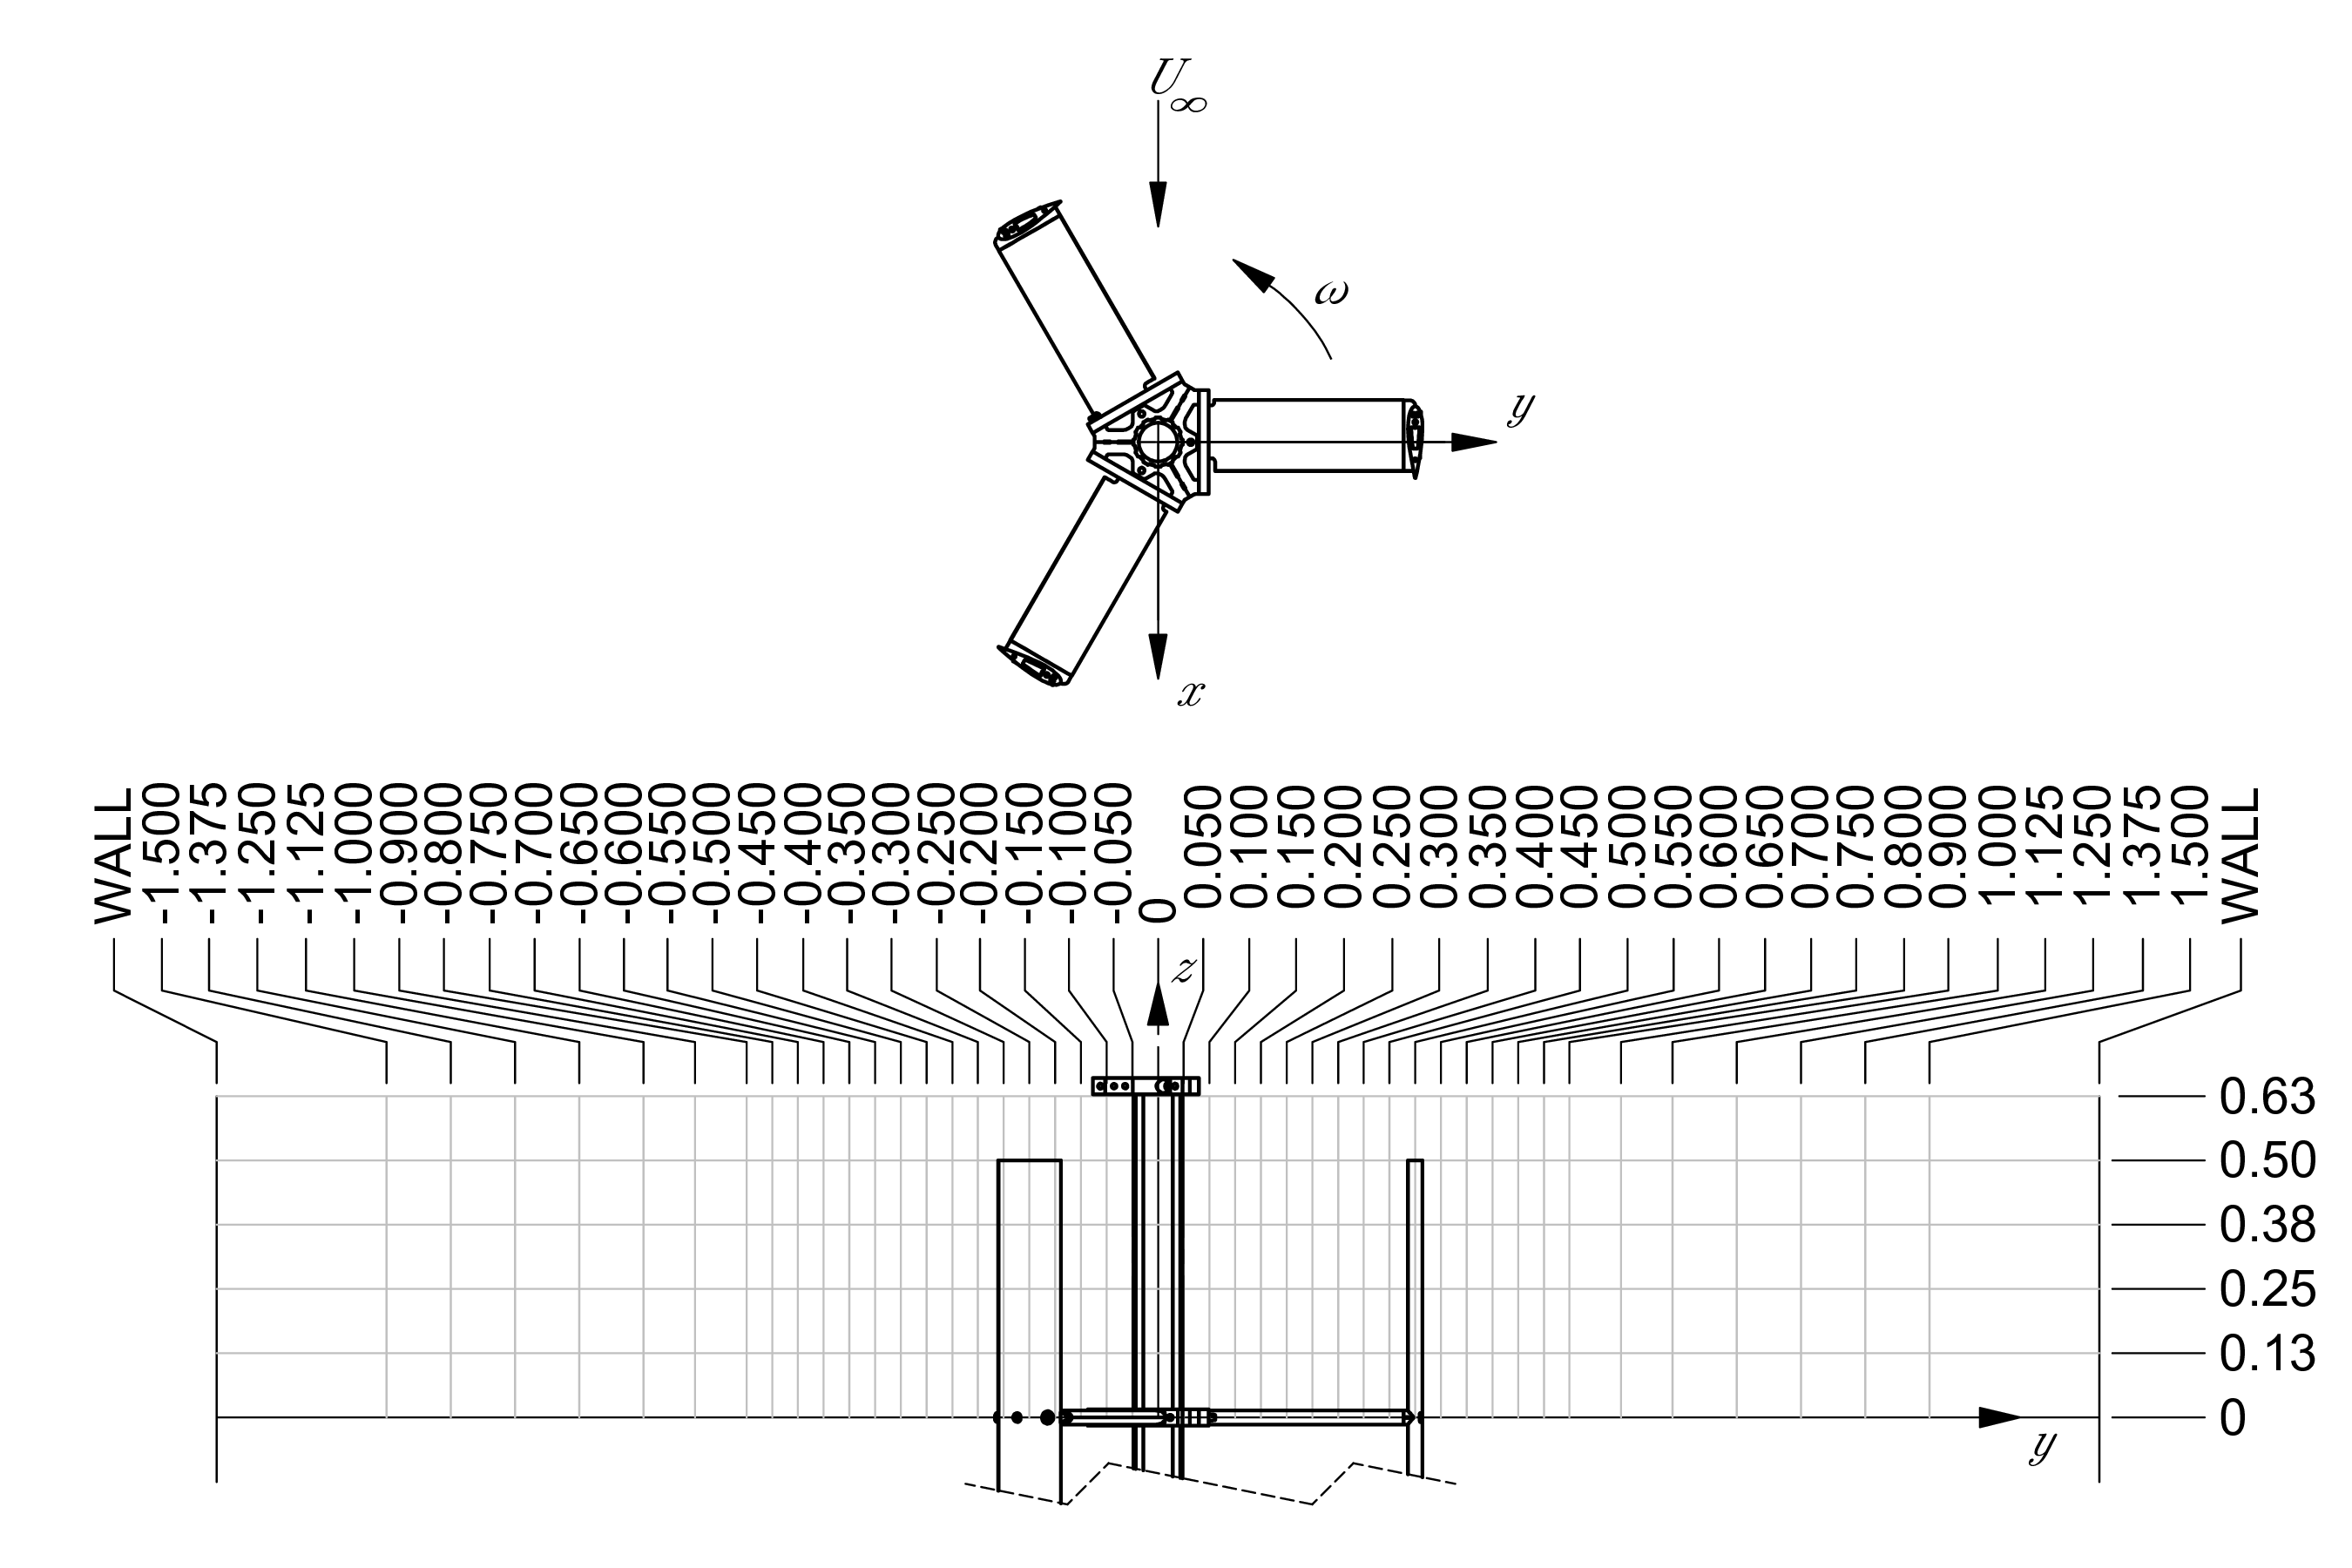
\includegraphics[width=0.9\textwidth]{unh-rvat-coord-sys}

    \caption{Wake measurement coordinate system and locations. Dimensions are in
        meters.}

    \label{fig:wake-locations}
\end{figure}


\subsection{Data processing}

From each set of tows, a standard time interval was set, which allowed the
turbine performance and wake to reach a quasi-periodic state. Each run was
analyzed to compute statistics over this interval, truncating the end slightly
to achieve an integer number of blade passages. Turbine shaft angular velocity
and tow carriage speed were calculated using a second order central differencing
scheme on the respective position measurements. Power and drag coefficients were
calculated as instantaneous quantities using the carriage speed as the free
stream velocity.

Wake velocity data were filtered for spurious ``spikes'' by removing data points
8 standard deviations, or 0.9 m/s, from the mean. The experimental data and code
for processing and visualization are available from
\cite{Bachant2016-RVAT-Re-dep}.


\subsection{Uncertainty}

Uncertainties from systematic and random error were estimated and combined using
the methods outlined in Section~\ref{sec:uncertainty}. For the Reynolds number
dependence of turbine performance, error bars are included on the plots.
Expanded uncertainty estimates for mean wake velocities (averaged over all runs)
are listed in Table~\ref{tab:vel-unc}.

\begin{table}[ht]
\centering
\begin{tabular}{c|c|c|c}
    $U_\infty$ (m/s) &   $U$ (m/s) &  $V$ (m/s) &  $W$ (m/s) \\
    \hline
    $0.4$ & $1 \times 10^{-2}$ & $7 \times 10^{-3}$ & $6 \times 10^{-3}$ \\
    $0.6$ & $1 \times 10^{-2}$ & $8 \times 10^{-3}$ & $8 \times 10^{-3}$ \\
    $0.8$ & $2 \times 10^{-2}$ & $1 \times 10^{-2}$ & $1 \times 10^{-2}$ \\
    $1.0$ & $2 \times 10^{-2}$ & $1 \times 10^{-2}$ & $1 \times 10^{-2}$ \\
    $1.2$ & $2 \times 10^{-2}$ & $1 \times 10^{-2}$ & $1 \times 10^{-2}$ \\
\end{tabular}
\caption{Average expanded uncertainty estimates (with 95\% confidence) for mean
    velocity measurements at each tow speed.}

\label{tab:vel-unc}
\end{table}


\section{Results and discussion}

\subsection{Performance}

Complete power and rotor drag (also known as thrust) coefficient curves for
various Reynolds numbers are plotted in Figures~\ref{fig:cp-curves} and
\ref{fig:cd-curves}, respectively. In general, maximum $C_P$ increases with
Reynolds number. The power coefficient curves also show a slight downward shift
in the optimal tip speed ratio (peak~performance) with increasing Reynolds
number, from about $\lambda \approx$ 2.0 to 1.9. This is caused by the stall
delay from a more turbulent boundary layer on the blade suction side. There is
essentially no change in the shape of the drag coefficient curves, merely a
slight upward shift in $C_D$ with increasing~ $Re$.

\begin{figure}
    \centering
    
    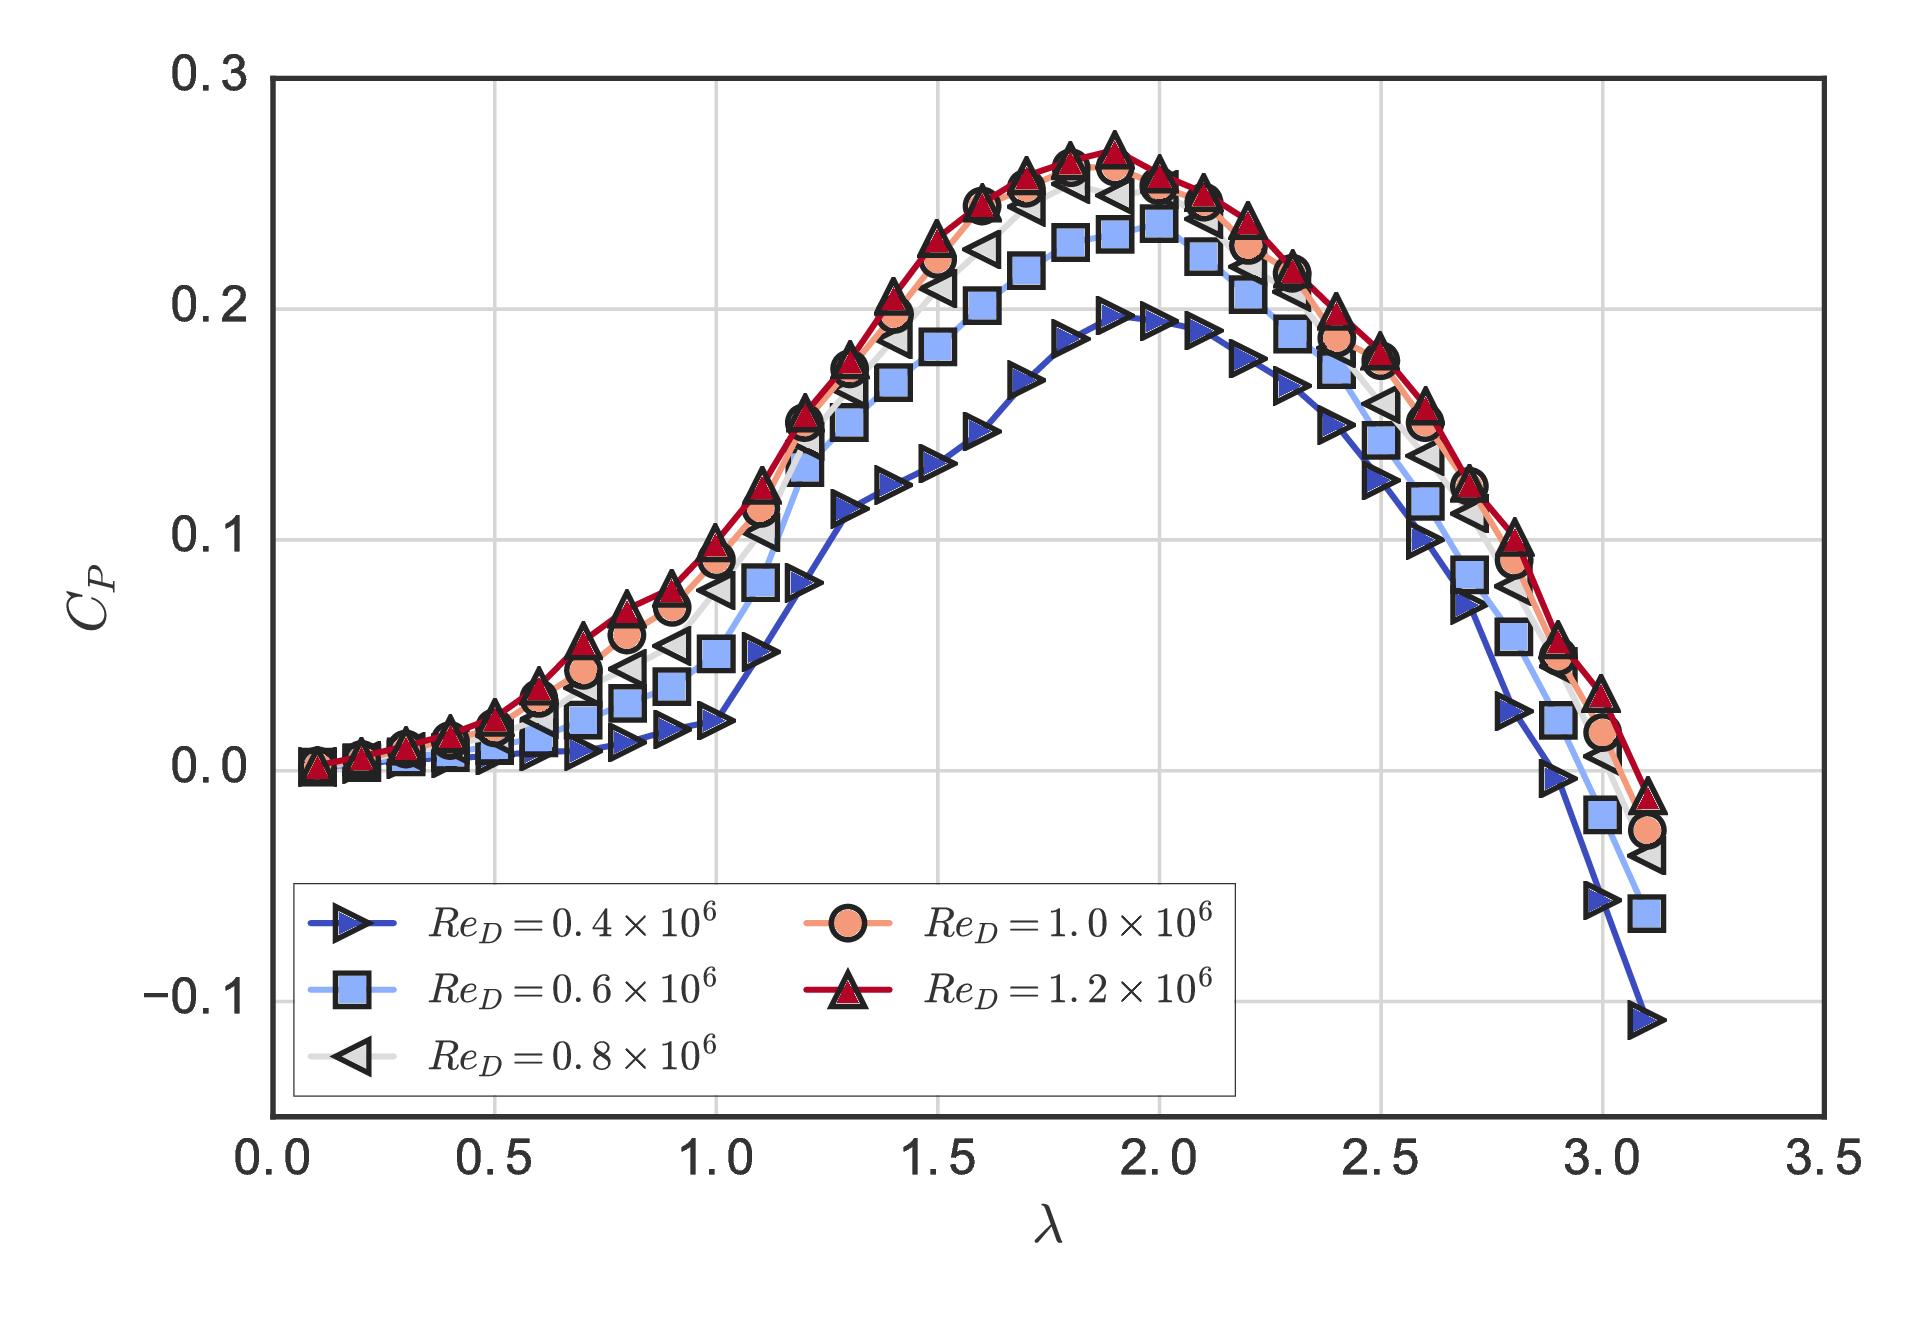
\includegraphics[width=0.75\textwidth]{RVAT-Re-dep_cp_curves}
    
    \caption{Mean power coefficient curves plotted for multiple Reynolds numbers.}
    
    \label{fig:cp-curves}
\end{figure}

\begin{figure}
    \centering
    
    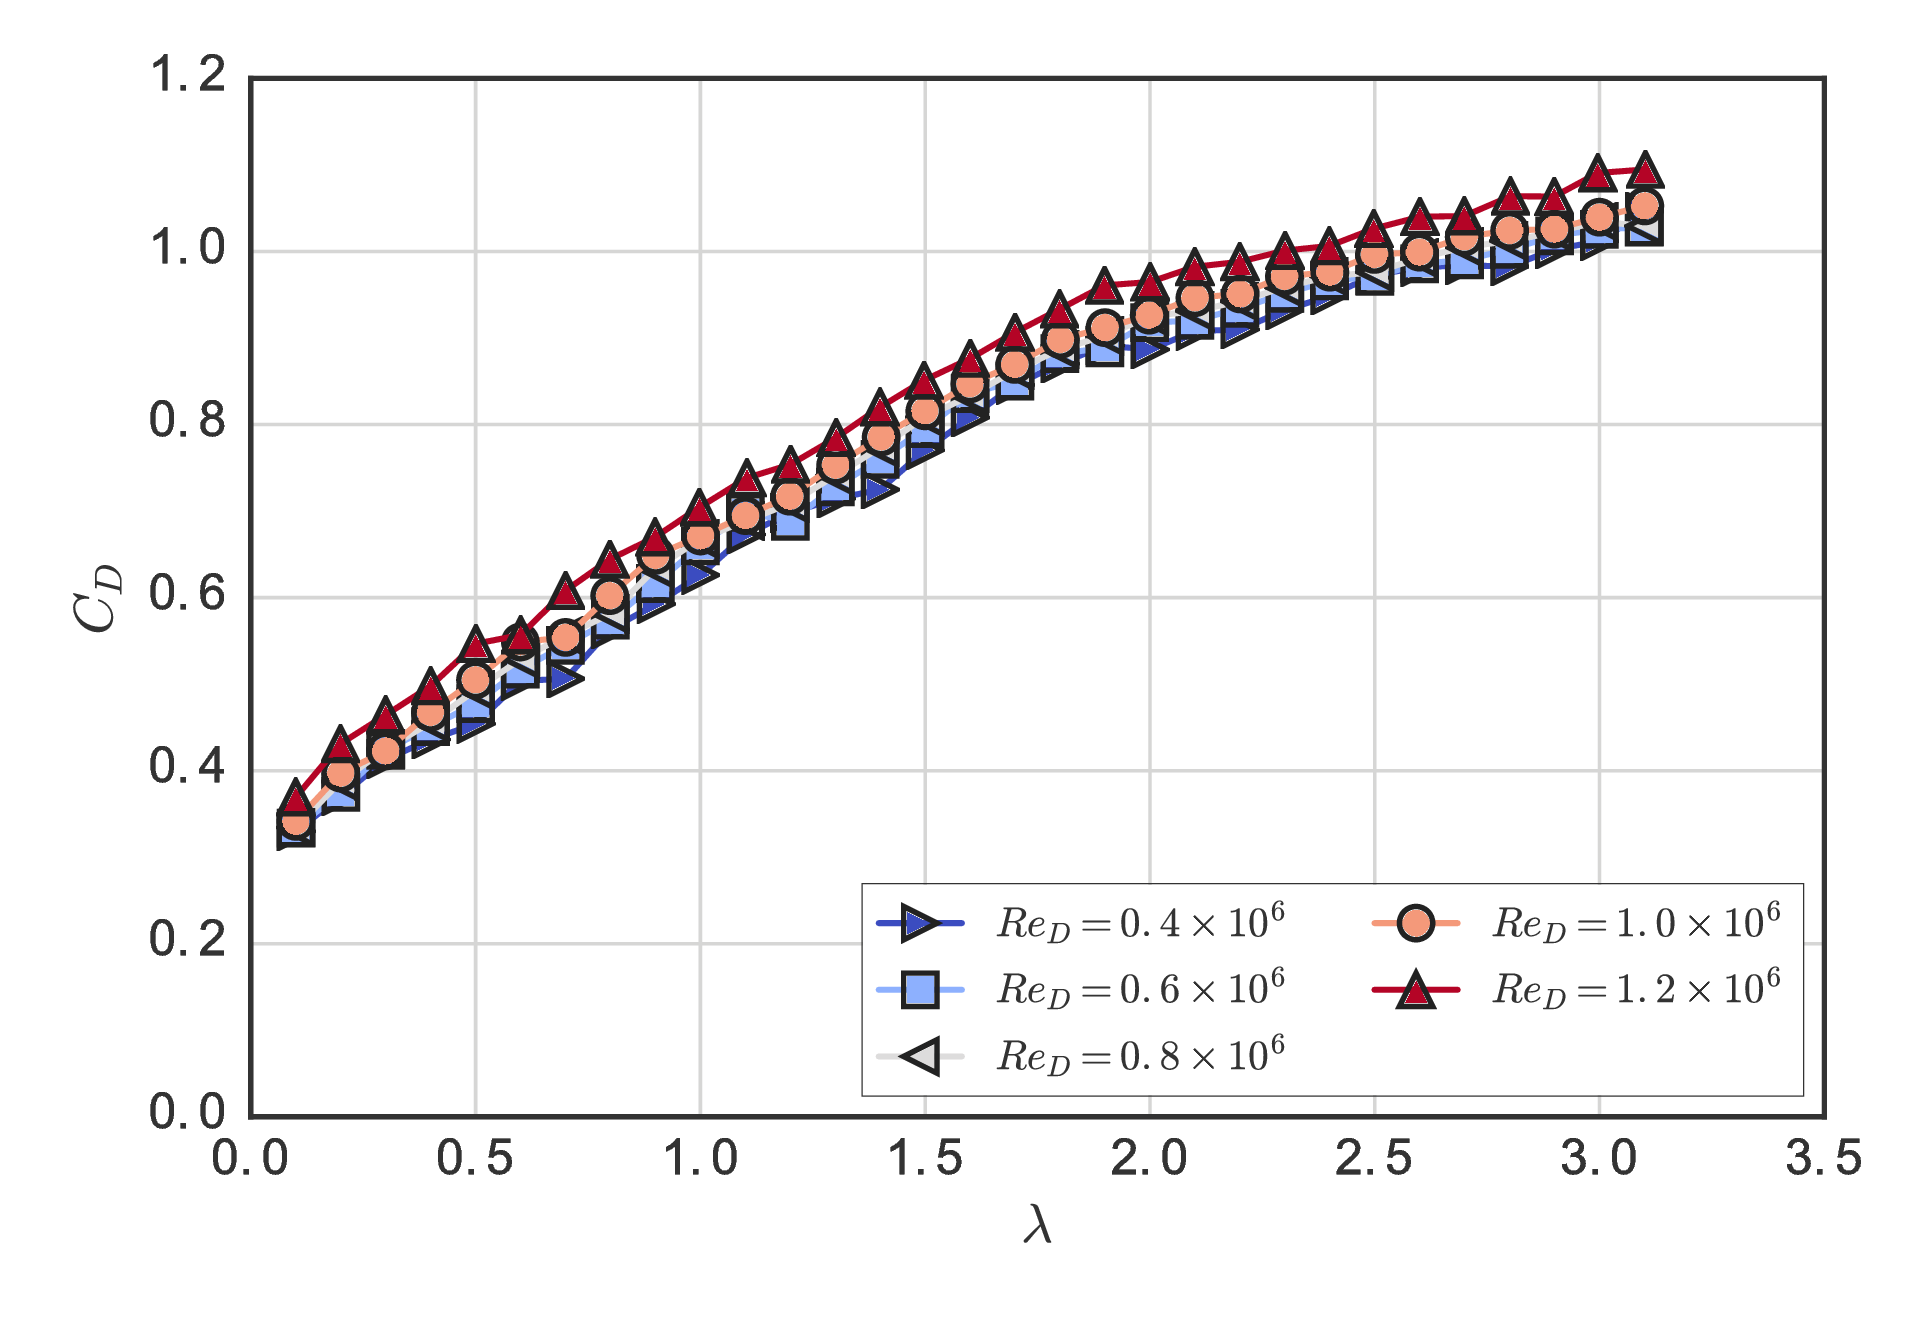
\includegraphics[width=0.75\textwidth]{RVAT-Re-dep_cd_curves}
    
    \caption{Mean rotor drag coefficient curves plotted for multiple Reynolds
        numbers.}
    
    \label{fig:cd-curves}
\end{figure}

Mean power and drag coefficients at $\lambda=1.9$ are plotted versus the
Reynolds number in Figure~\ref{fig:perf-Re-dep}. Note that the large error bars
for $C_P$ at low $Re$ are dominated by systematic error estimates for the torque
transducer, since torque values are at the lower end of its measurement range.
However, the uncertainty due to random error or repeatability remains relatively
low. There is a drastic improvement in $C_P$ with increasing Reynolds number at
the lower end of the $Re$ range. The power coefficient then becomes essentially
$Re$-independent at $Re_D = 0.8 \times 10^6$, which corresponds to an
approximate average blade chord Reynolds number $Re_{c, \mathrm{ave}} = 2.1
\times 10^5$. This threshold is consistent with the behavior of the blade
boundary layer transitioning from laminar to turbulent, thereby promoting either
the suppression or reattachment of the laminar separation bubble
\cite{Lissaman1983}.


\begin{figure}
    \centering
    
    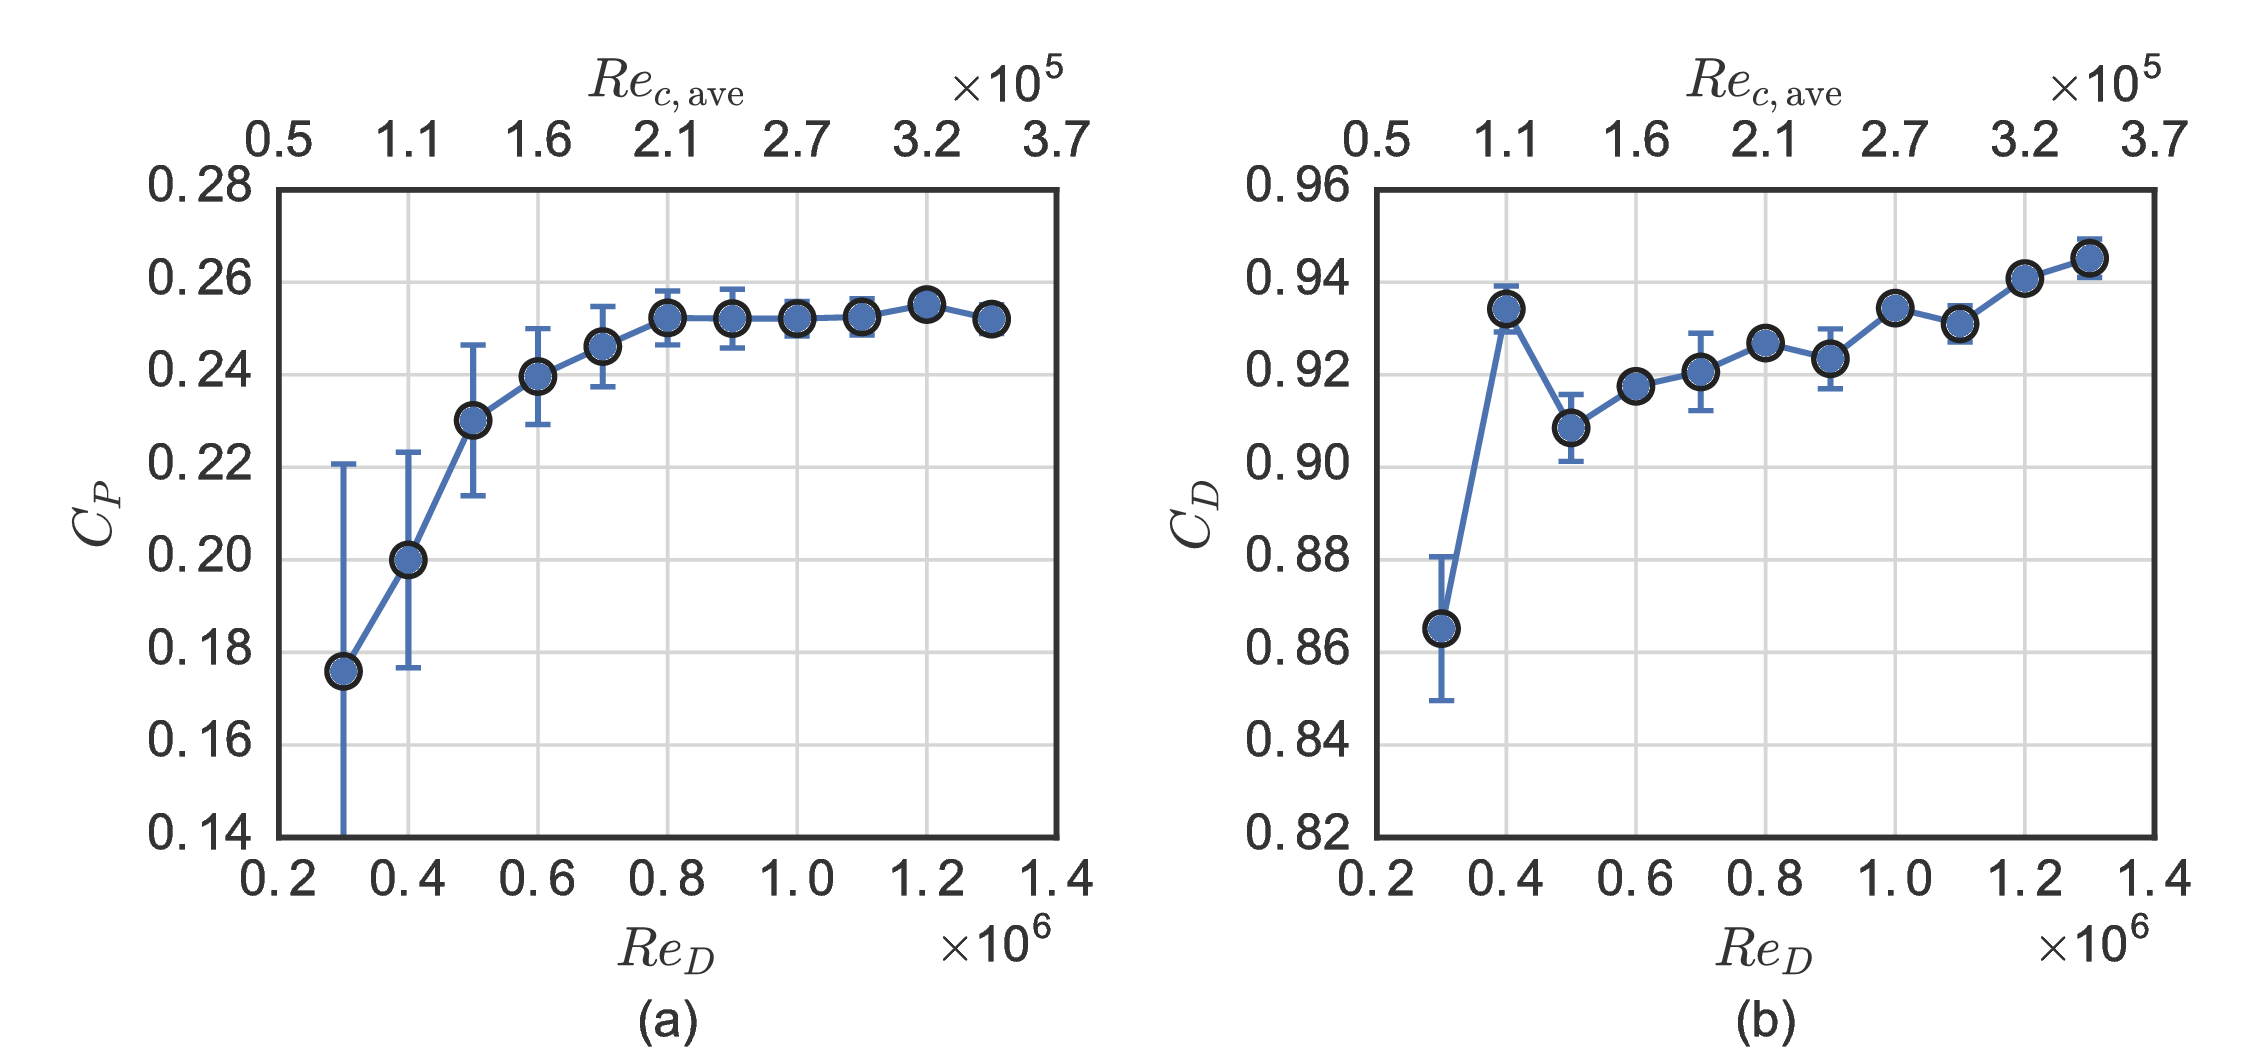
\includegraphics[width=0.9\textwidth]{RVAT-Re-dep_perf_re_dep}
    
    \caption{UNH-RVAT measured mean (a) power and (b) drag coefficients at
        $\lambda=1.9$ plotted versus the Reynolds number. Error bars indicate
        expanded uncertainty estimates for 95\% confidence, which for $C_P$ is dominated
        by systematic error estimates from the torque transducer operating at the lower
        end of its measurement range.}
    
    \label{fig:perf-Re-dep}
\end{figure}

The behavior of the mean rotor drag coefficient $C_D$ is similar, though the
changes are less dramatic. This is likely due to cross-flow turbine geometry,
where increases in blade drag at lower $Re$ somewhat offset the reduction in
lift, causing the total streamwise force to vary less than the rotor torque.
The tendency for $C_D$ to continue increasing with $Re$ may also include the
effects of an increasing Froude number (from faster tow speeds), which increases
free surface deformation and wave drag during towing without increasing flow
through the turbine.


\subsubsection{Relation to static foil characteristics}

To help understand, and possibly predict, the $Re$-sensitivity on turbine
performance, a series of static foil coefficient datasets were computed with the
viscous panel method code XFOIL \cite{Drela1989}, a commonly-used tool for
airfoil analysis, e.g., \cite{Castelli2011, Walker2014}, implemented as part of
the open source turbine design software QBlade \cite{Marten2013}. Simulations
were run for an angle of attack range of 0$^{\circ}$ to 40$^{\circ}$, in
increments of 0.5$^{\circ}$. Solver parameters used were 100 panels, a fixed
speed, zero Mach number, \texttt{NCrit=9} (default $\mathrm{e}^n$ transition
criteria parameter for an average wind tunnel), and no forced boundary layer
transition. Characteristics were computed for the approximate average blade
chord Reynolds numbers encountered in the tow tank experiments.

To investigate the effects of the blades' ``virtual camber'' due to their
circular path \cite{Migliore1980}, the XFOIL calculations were performed for
20\% thick foils with 0\% (NACA 0020), 2\% (NACA 2520), and 4\% (NACA 4520)
camber about their half-chord location. A 4\% camber approximates the maximum
distance between the blade chord line and path for the UNH-RVAT, and the 2\%
camber takes into account the reduction in virtual flow curvature from the
non-curved inflow velocity by dividing by the tip speed ratio $\lambda=1.9$.

Results from the XFOIL calculations for the airfoil profiles are shown in
Figure~\ref{fig:foil-Re-dep}, where values of the maximum lift coefficient
$C_{l_{\max}}$, minimum drag coefficient $C_{d_{\min}}$, and maximum
lift-to-drag ratio are normalized (to visualize relative differences in scaling
between the foils) and plotted versus $Re_c$. In general, larger camber
is associated with decreased foil performance at lower Reynolds number. The data
and processing code for these calculations is available from
\cite{Bachant2016-NACAXX20-XFOIL}.

\begin{figure}
    \centering
    
    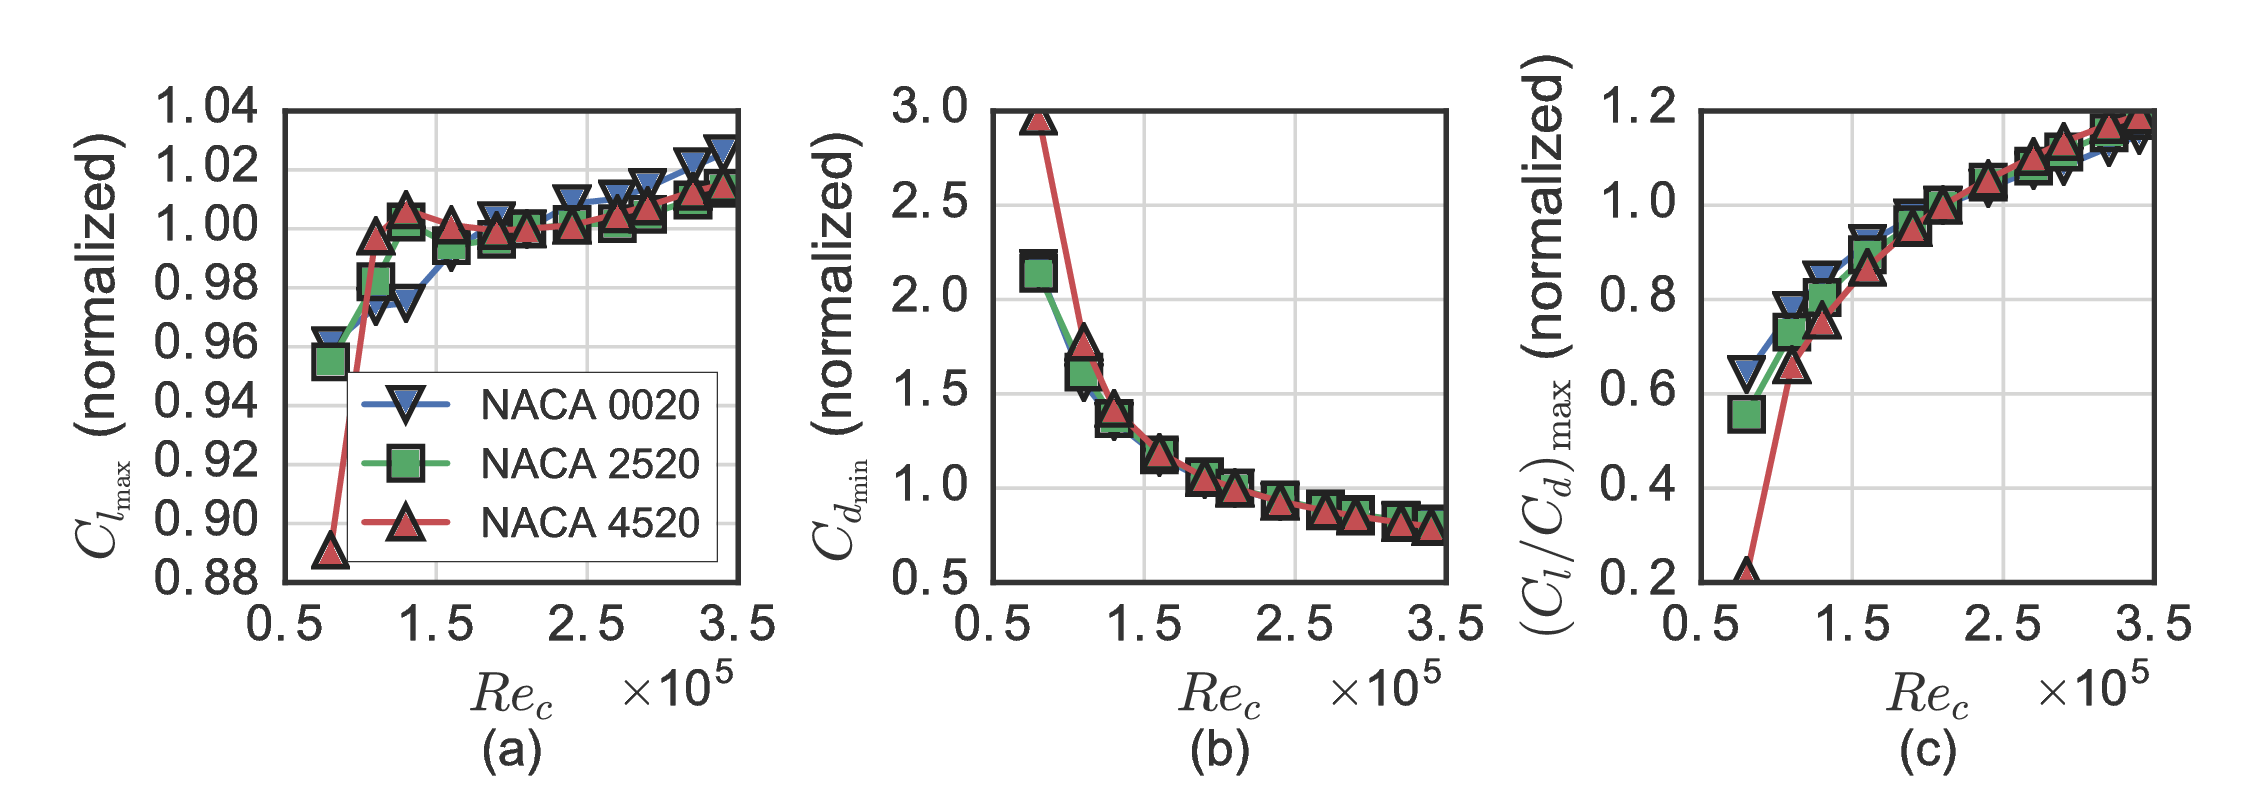
\includegraphics[width=0.95\textwidth]{NACAXX20-XFOIL_all_foils_re_dep}
    
    \caption{Normalized maximum (a) lift coefficient, (b) drag coefficient, and
        (c) lift-to-drag ratio computed by XFOIL at various $Re_c$  for each
        profile.}
    
    \label{fig:foil-Re-dep}
\end{figure}

In conjunction with the cross-flow turbine blade kinematics, the foil
coefficients were used to approximate turbine performance by calculating the
peak torque coefficient on the upstream half of the blade path. The turbine
torque coefficient $C_T$ can be related to the blade section chordwise force
coefficient $C_c$ by:
\begin{equation}
    C_T = \frac{C_c c}{2R} \frac{|U_\mathrm{rel}|^2}{U_\infty^2},
    \label{eq:ct}
\end{equation}
where the blade section chordwise force coefficient (for zero preset pitch) is
given by:
\begin{equation}
    C_c = C_l \sin \alpha - C_d \cos \alpha.
    \label{eq:cc}
\end{equation}

The relative blade velocity $U_\mathrm{rel}$ was calculated by vector addition
of the free stream velocity and the opposite of the blade tangential velocity.
Note that this neglects any induction, \emph{i.e.}, slowing of the free stream
by the turbine forces, which would be present in a momentum/streamtube model.
Since~the goal of this approach was not to predict absolute performance, but
rather to gain insight into relative changes with $Re$, this method was deemed
acceptable, as it is extremely simple and fast to~compute.

Values for the blade angle of attack, relative velocity, and torque coefficient
are plotted in Figure~\ref{fig:blade-kinematics} for the upstream half of
rotation of the turbine. The effects of static stall are clearly present in the
torque coefficient plot, and by the time the angle of attack has decreased below
the static stall angle, the relative velocity is so low that there is not much
contribution to the torque coefficient.

\begin{figure}
    \centering
    
    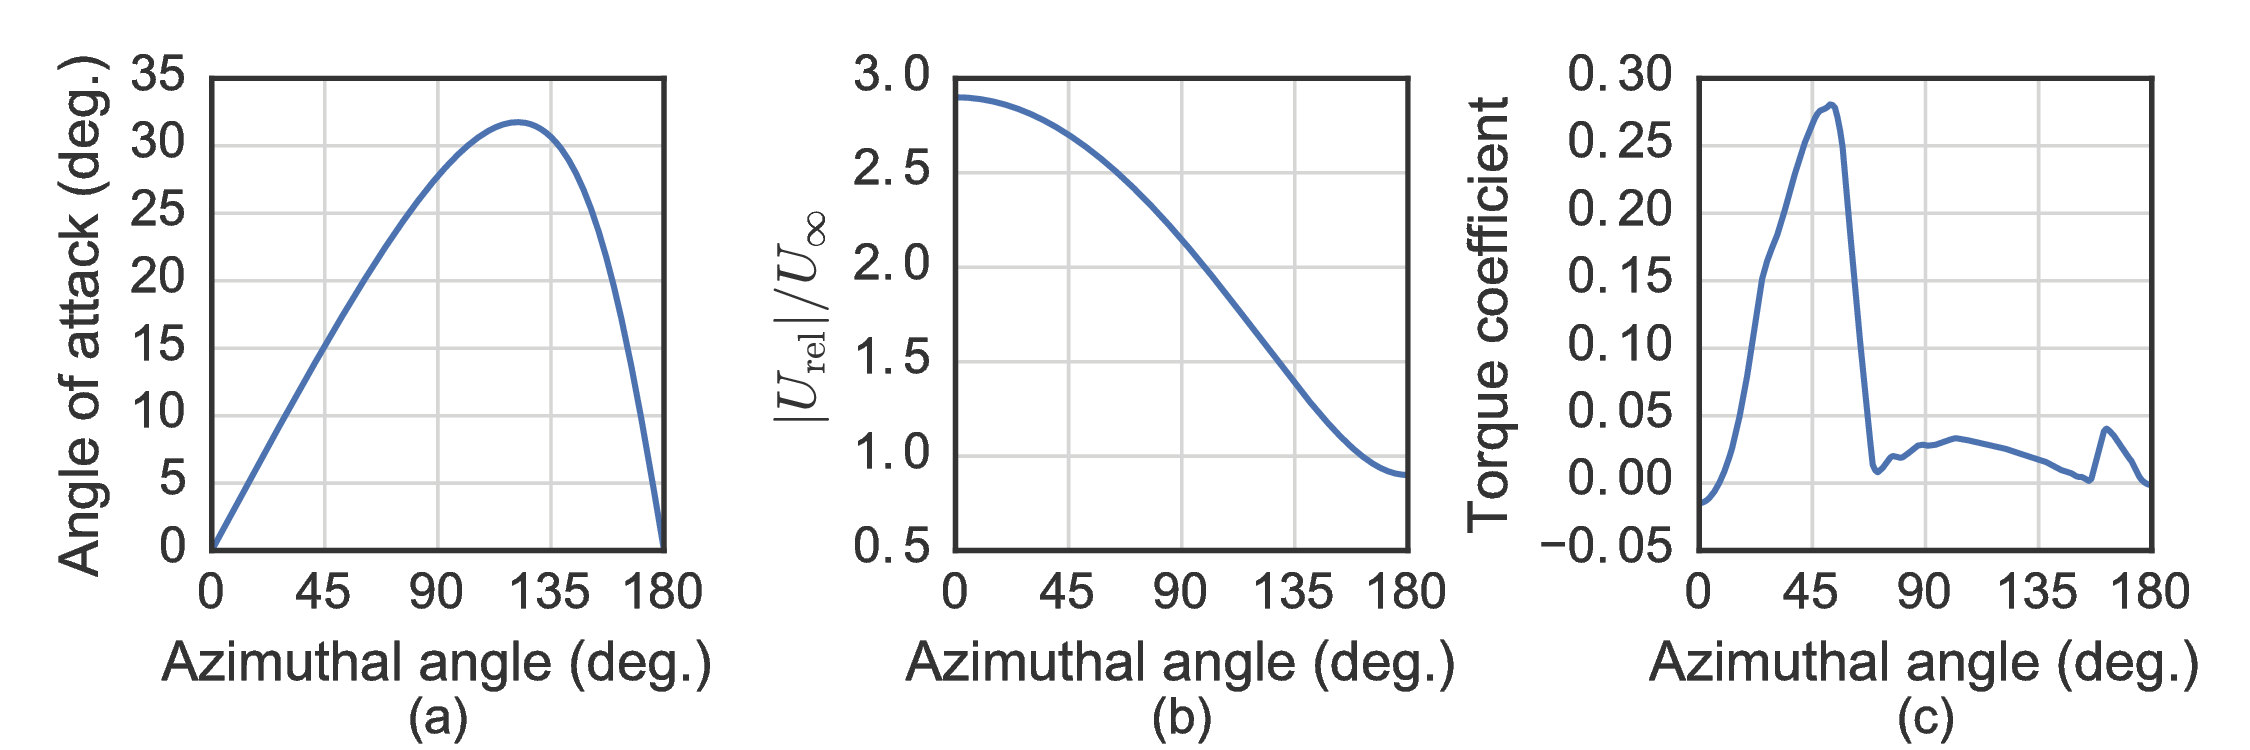
\includegraphics[width=0.95\textwidth]{NACAXX20-XFOIL_foil_kinematics_ct}
    
    \caption{Geometric (a) angle of attack, (b) relative velocity , and (c)
        torque coefficient calculated with a NACA 0020 foil operating at
        $\lambda=1.9$.}
    
    \label{fig:blade-kinematics}
\end{figure}

Results for the normalized peak torque coefficient for each foil are plotted
versus $Re_c$ in Figure~\ref{fig:foils-C_T-Re-dep}. It is interesting
that the convergence of $C_{T_\mathrm{max}}$ with increasing Reynolds number is
more dramatic than any of the common foil performance characteristics plotted in
Figure~\ref{fig:foil-Re-dep}, meaning that the cross-flow turbine's unique
kinematics must be taken into account when attempting to predict the effect of
transitional Reynolds numbers on turbine performance.

From the peak torque coefficient metric plotted in
Figure~\ref{fig:foils-C_T-Re-dep}, the Reynolds number independence is achieved
at lower values and more dramatically. We see that the trend of the
(non-cambered) NACA 0020 curve matches almost perfectly up to $Re_c \approx 2.1
\times 10^5$, but then continues to increase slowly and linearly with $Re$. This
is not matched by the experimental data, which at higher $Re$ looks more like
the cambered foil results. Though this method does not provide absolute
predictions of turbine performance, it predicts the transitional Reynolds number
regime for cross-flow turbine performance using only 2D static airfoil
characteristics, \emph{i.e.}, the Reynolds number scaling of the peak $C_T$
computed this way behaves much like that of the measured turbine performance.

\begin{figure}
    \centering
    
    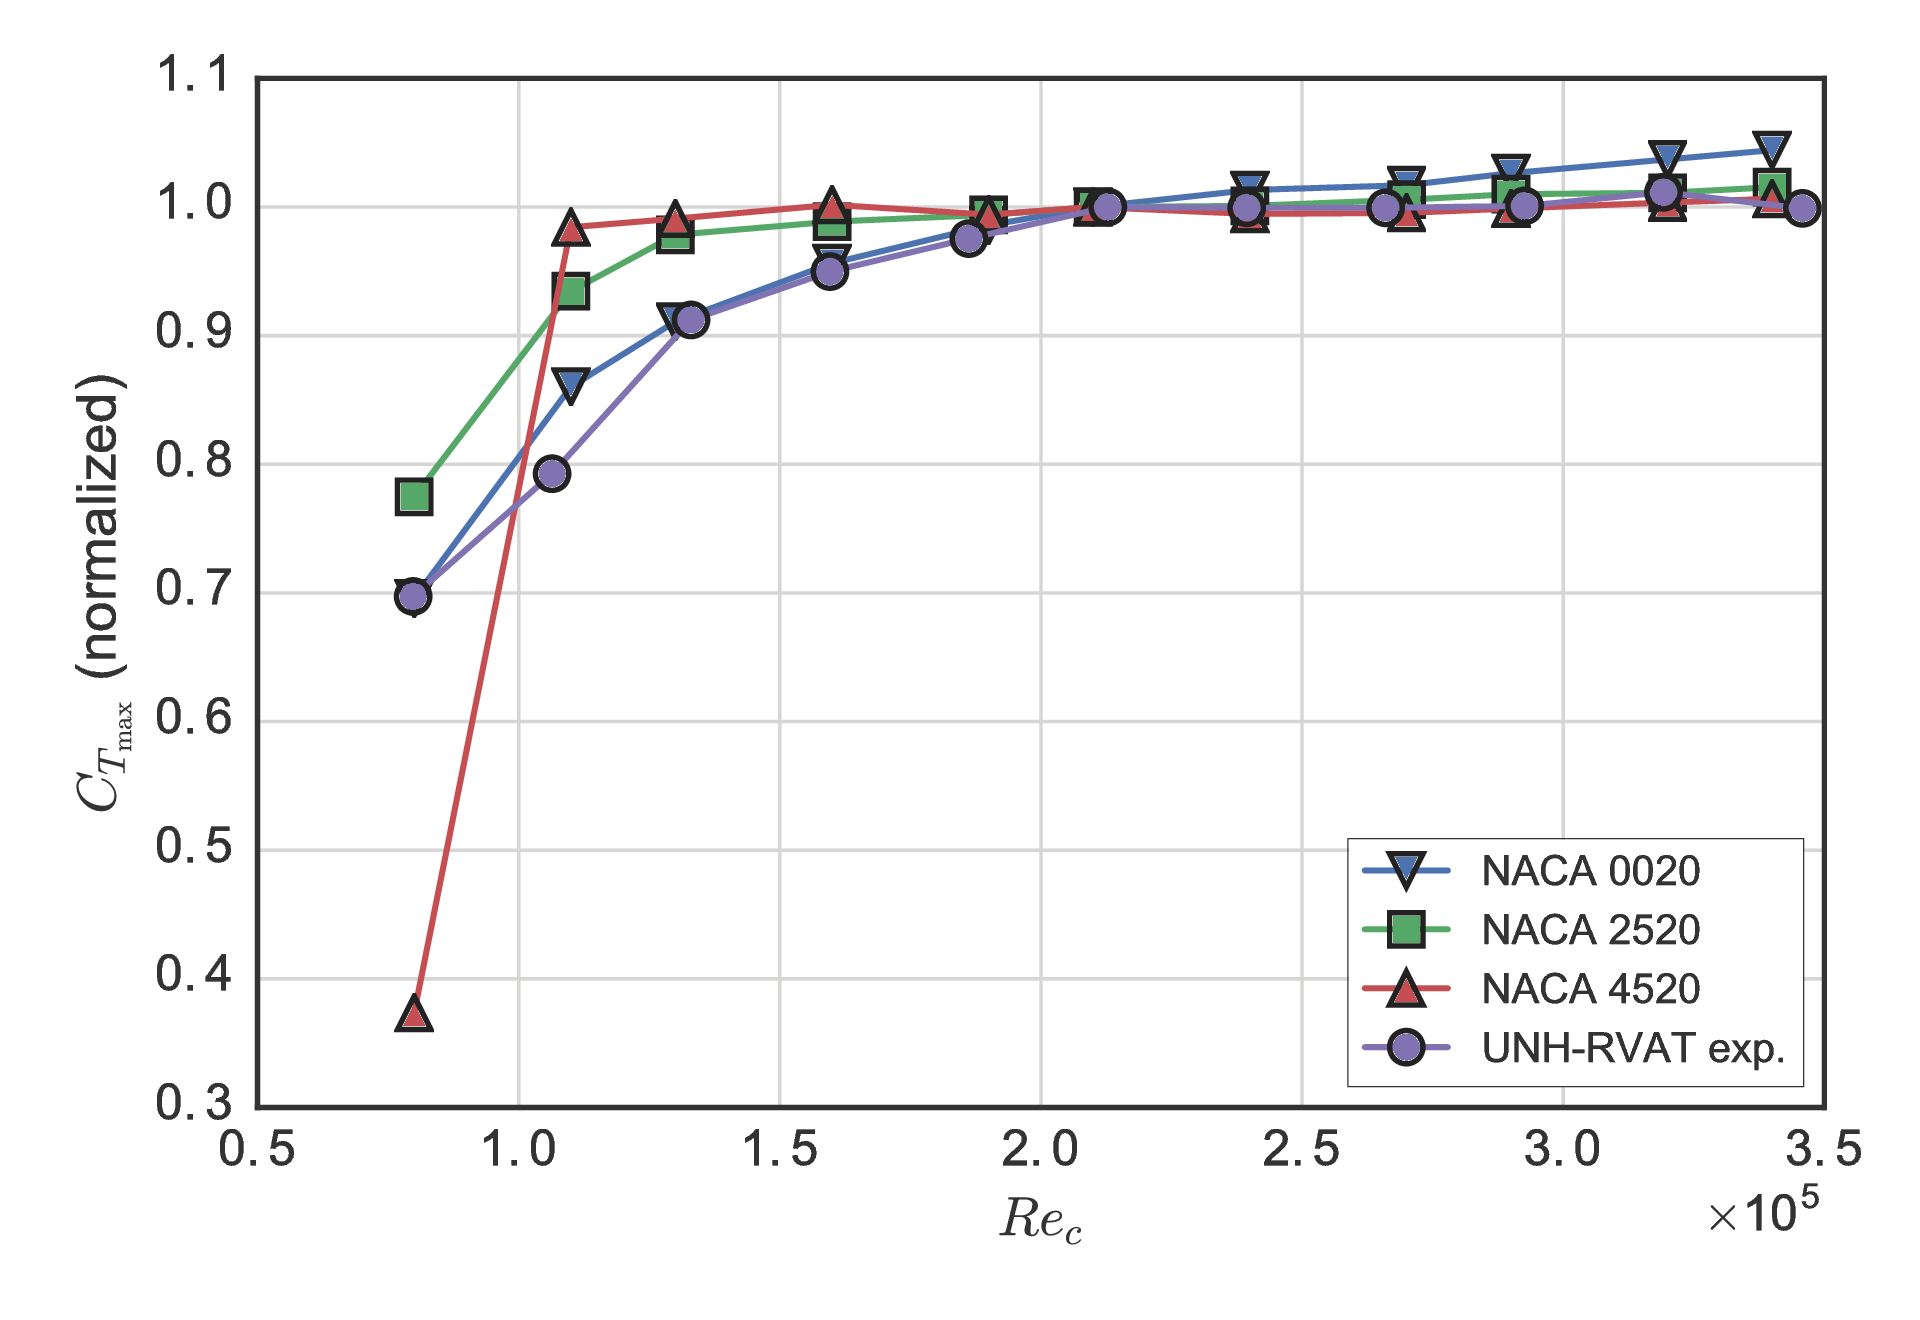
\includegraphics[width=0.75\textwidth]{NACAXX20-XFOIL_cft_re_dep_foils}
    
    \caption{Reynolds number dependence of the normalized peak torque
        coefficient calculated from static foil coefficients and blade kinematics,
        compared to experimental data from a cross-flow turbine. Note that the
        experimental data represents the mean torque coefficient, not the maximum.}
    
    \label{fig:foils-C_T-Re-dep}
\end{figure}


\subsection{Wake characteristics}

The near-wake of this turbine at $x/D=1$, $\lambda=1.9$, along with momentum and
kinetic energy balances at a $Re_D = 1.0 \times 10^6$ were discussed in
\cite{Bachant2015-JoT}. Similar data were taken for the experiment here, and the
results for the mean velocity field and turbulence kinetic energy calculated
from wake maps of 270 individual measurements (tows) are shown in
Figures~\ref{fig:meancontquiv} and \ref{fig:kcont}, respectively, looking
upstream towards the turbine. With respect to the mean velocity field, we see
asymmetry and a mean vortex structure created by blade tip vortex shedding. The
effects of the tip vortices are also seen in the turbulence kinetic energy
measurements, along with turbulence generated by the blades undergoing dynamic
stall on the $-y$ side of the turbine.

These same wake maps were measured for $Re_D = 0.4 \times 10^6$, $0.6 \times
10^6$, $0.8 \times 10^6$, and $1.2 \times 10^6$. Qualitatively, these look very
similar, so they have not been plotted here, though profiles at $z/H=0.0$ are
compared in Figure~\ref{fig:profiles} to illustrate the subtlety of the
differences at different $Re$. We will instead compare and contrast the wake
behavior by examining spectra and wake transport terms in the equations that
govern the downstream evolution of mean momentum and kinetic energy.

\begin{figure}
    \centering
    
    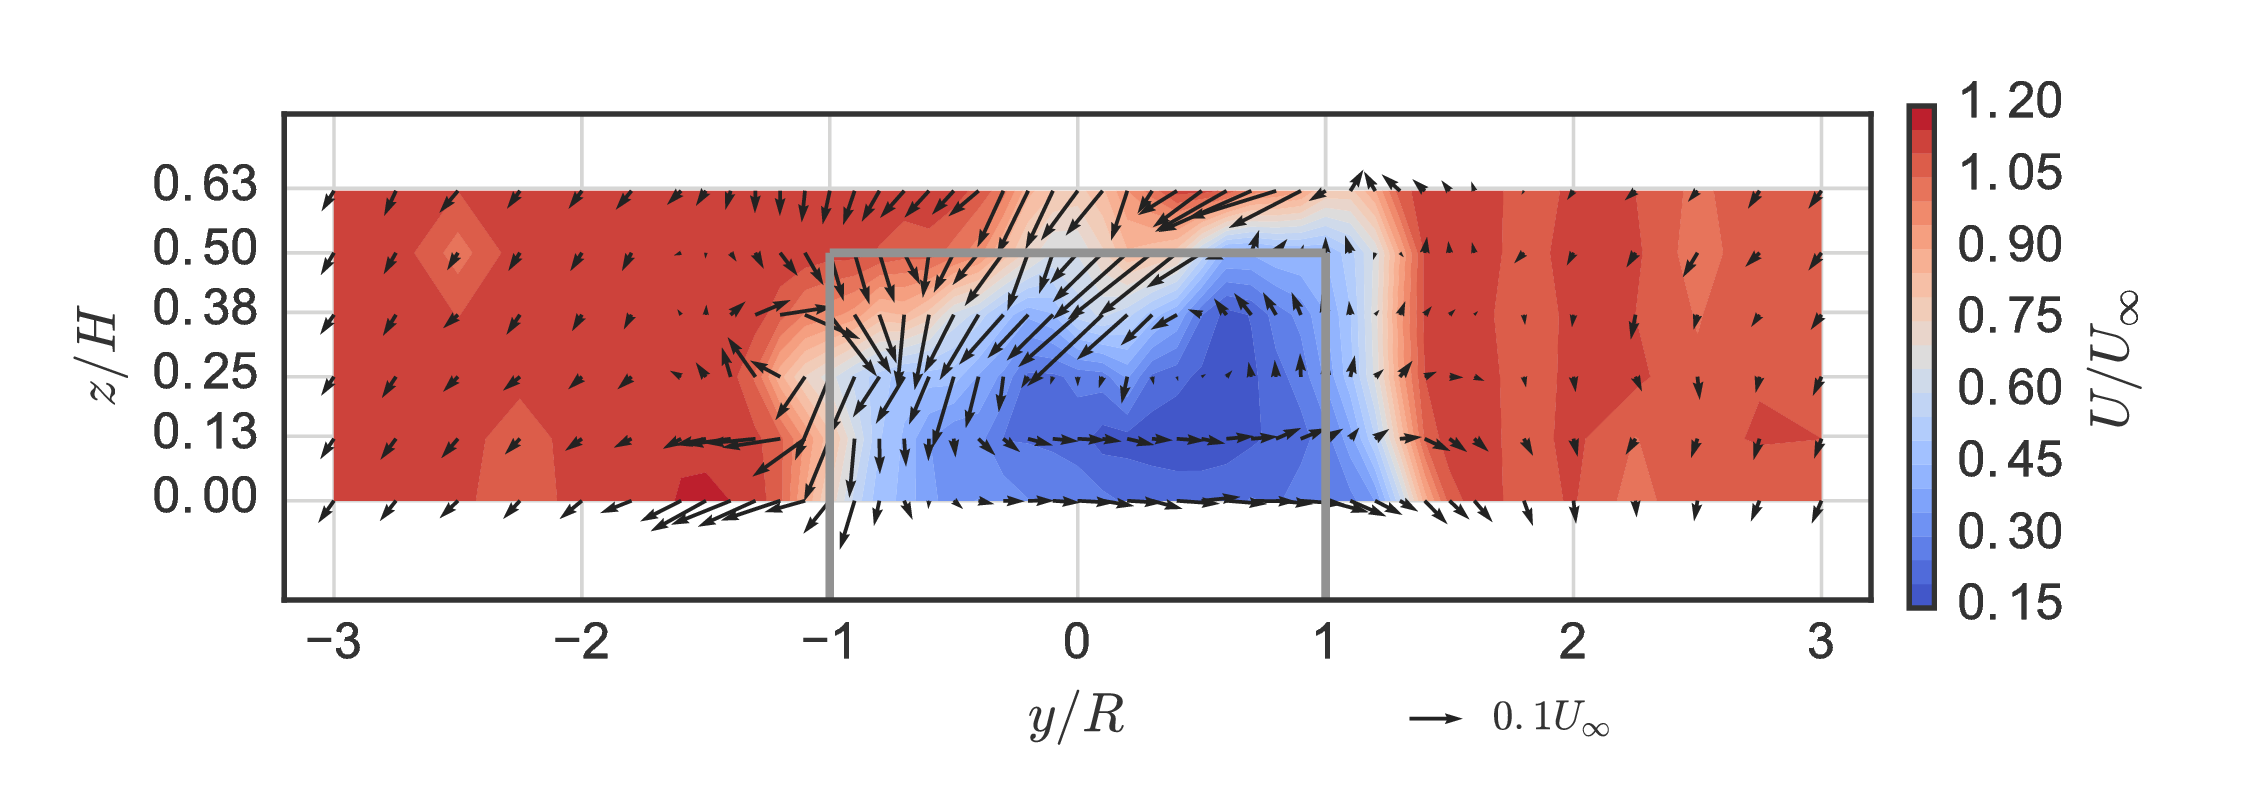
\includegraphics[width=0.85\textwidth]{RVAT-Re-dep_meancontquiv_10}
    
    \caption{Mean velocity field at $x/D=1$, $\lambda=1.9$, and $Re_D=1.0 \times
        10^6$.}
    
    \label{fig:meancontquiv}
\end{figure}

\begin{figure}
    \centering
    
    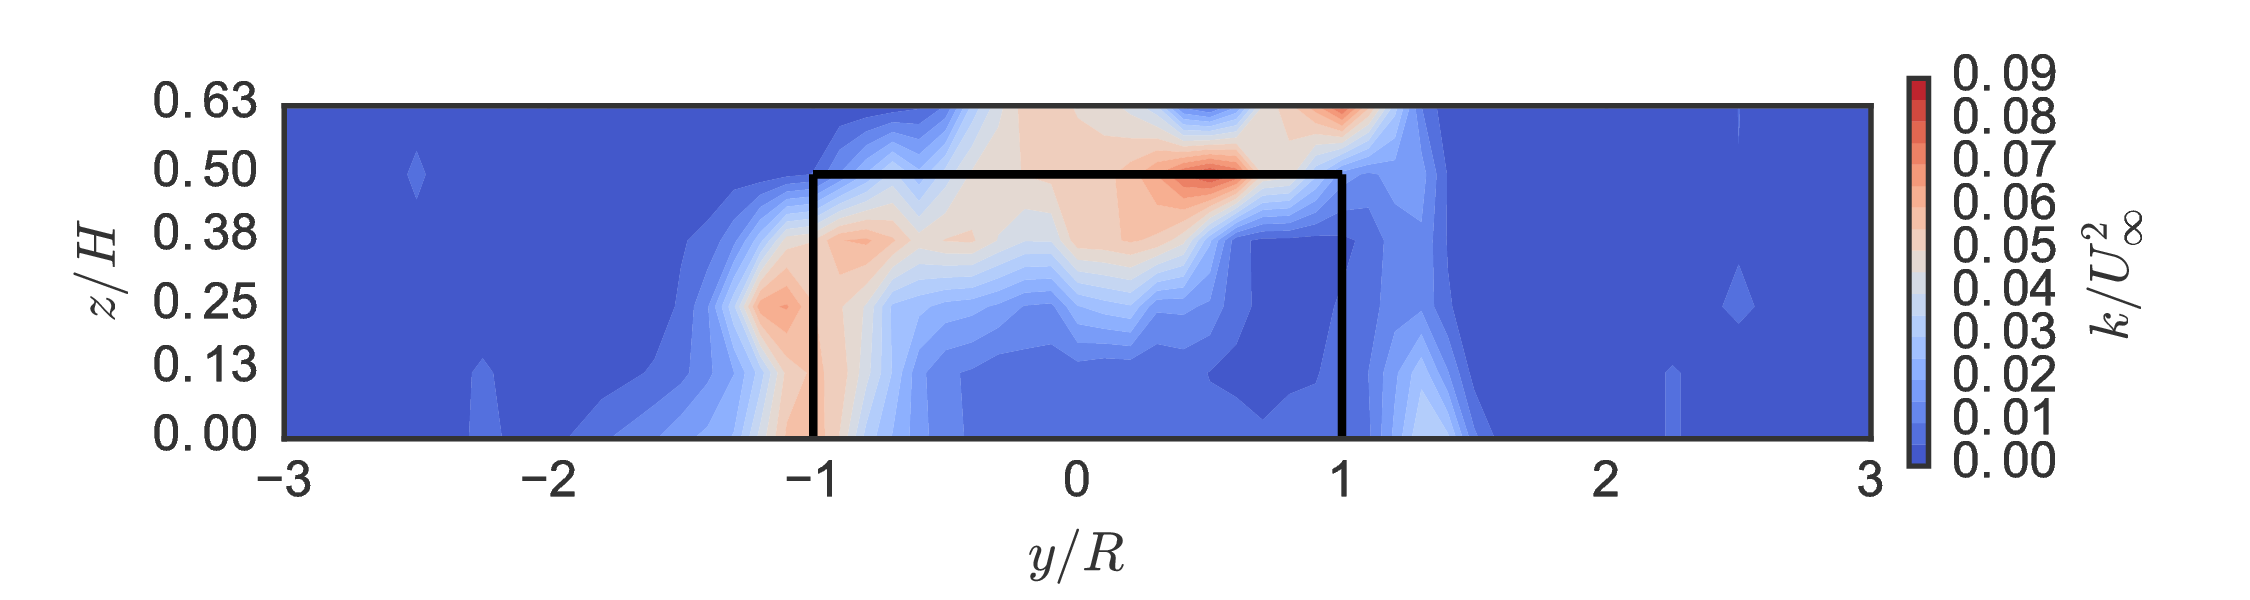
\includegraphics[width=0.85\textwidth]{RVAT-Re-dep_k_contours_10}
    
    \caption{Turbulence kinetic energy at $x/D=1$, $\lambda=1.9$, and $Re_D=1.0
        \times 10^6$.}
    
    \label{fig:kcont}
\end{figure}

\begin{figure}[ht]
    \centering
    
    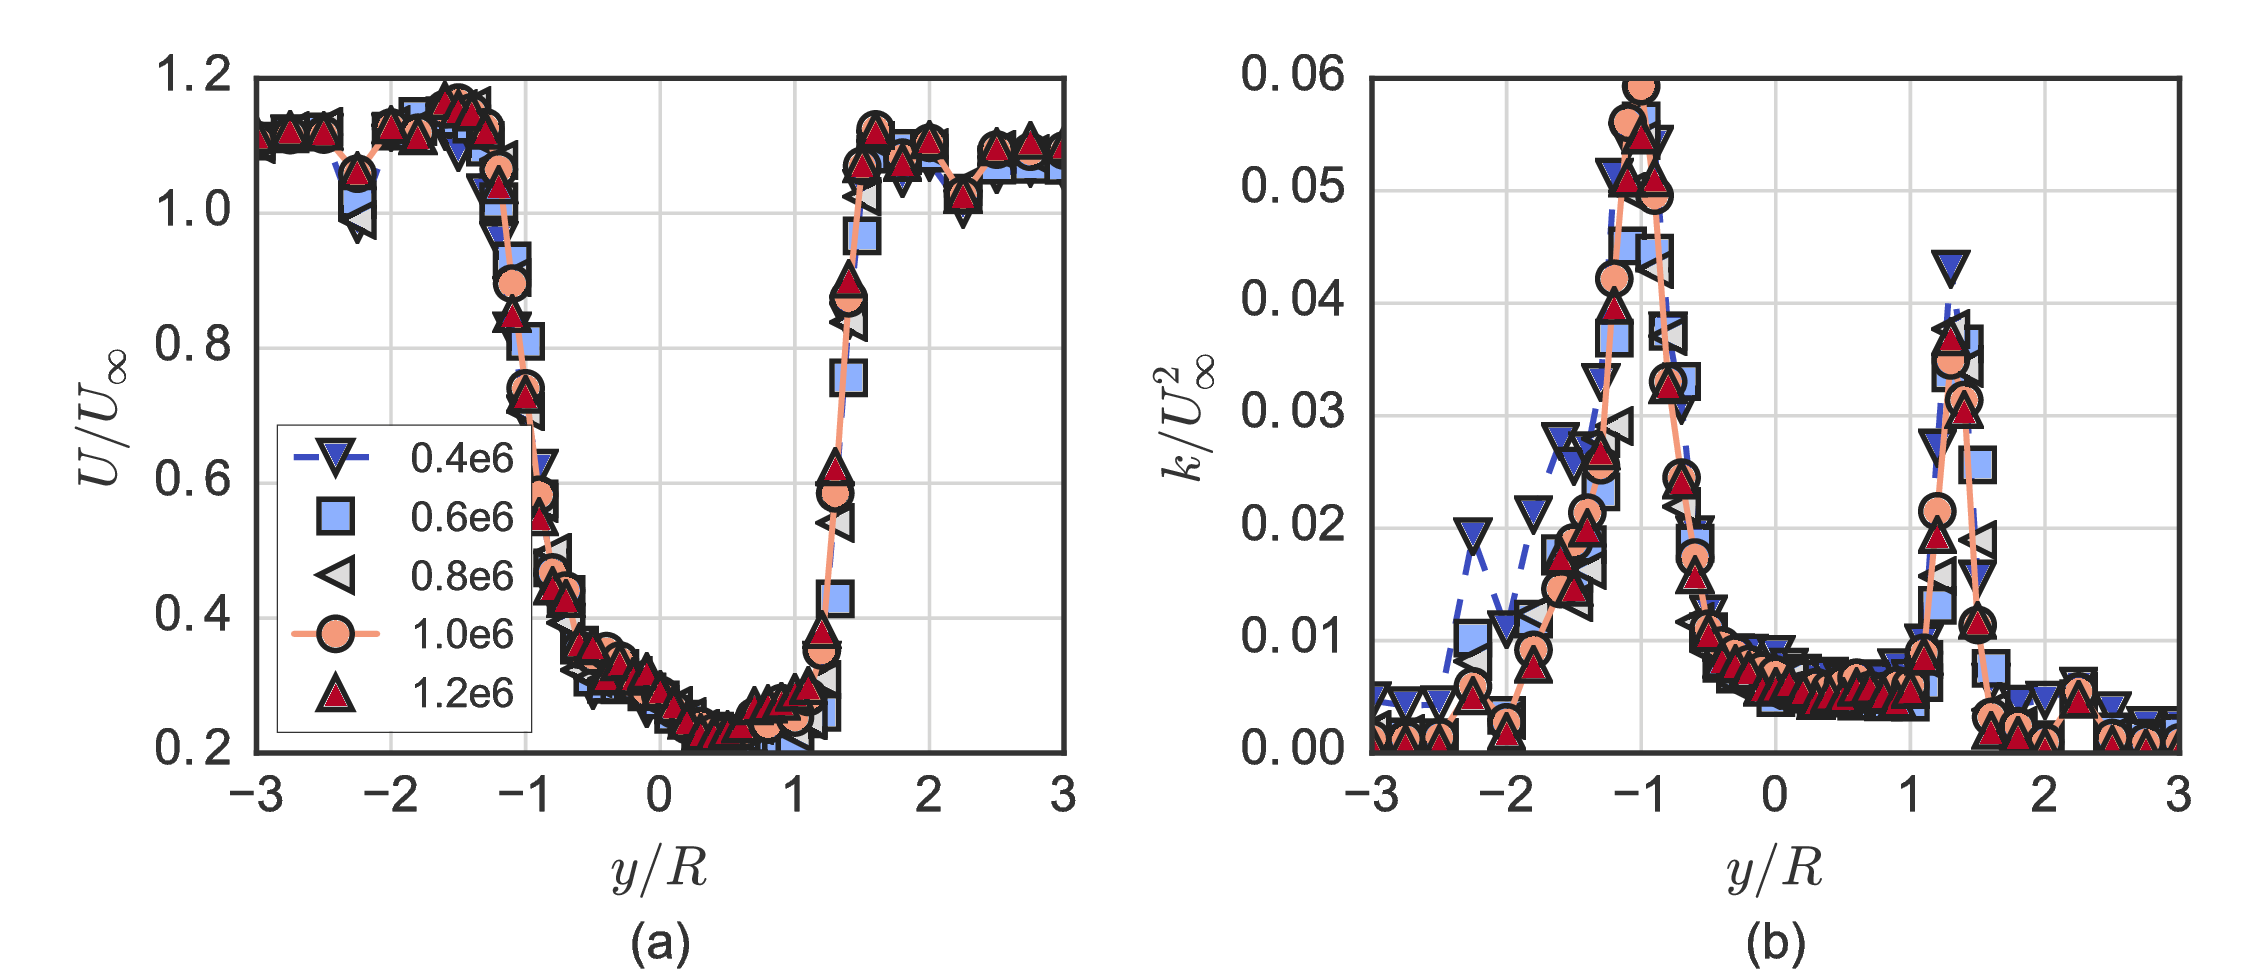
\includegraphics[width=0.9\textwidth]{RVAT-Re-dep_mean_u_k_profiles}
    
    \caption{Mean streamwise velocity (a) and turbulence kinetic energy (b)
        profiles at $z/H=0.0$. Turbine diameter Reynolds number $Re_D$ is indicated
        by the legend.}
    
    \label{fig:profiles}
\end{figure}

\todo[inline]{Profiles fig should have legend in lower left.}


\subsubsection{Dominant timescales and turbulence spectra}

Spectra of the cross-stream velocity normalized by the free stream were computed
using a fast Fourier transform-based method, applying a Hanning window and
averaging over four adjacent frequency bands to decrease confidence intervals.
These spectra are plotted in Figure~\ref{fig:wake-spectra} for regions on either
side of the turbine. On the $-y$ side of the turbine, there is broadband
turbulence produced by blade stall, and on the $+y$ side, there is a clear peak
in the spectra caused by the blade passage. We see that on both sides, there is
higher spectral energy at lower Reynolds numbers. On the $+y$ side of the
turbine, we notice higher spectral energy at the blade passage frequency's first
harmonic, or $6 f_\mathrm{turbine}$. This is likely due to the blade's shed
vorticity being less stable at higher $Re$.

\begin{figure}
    \centering
    
    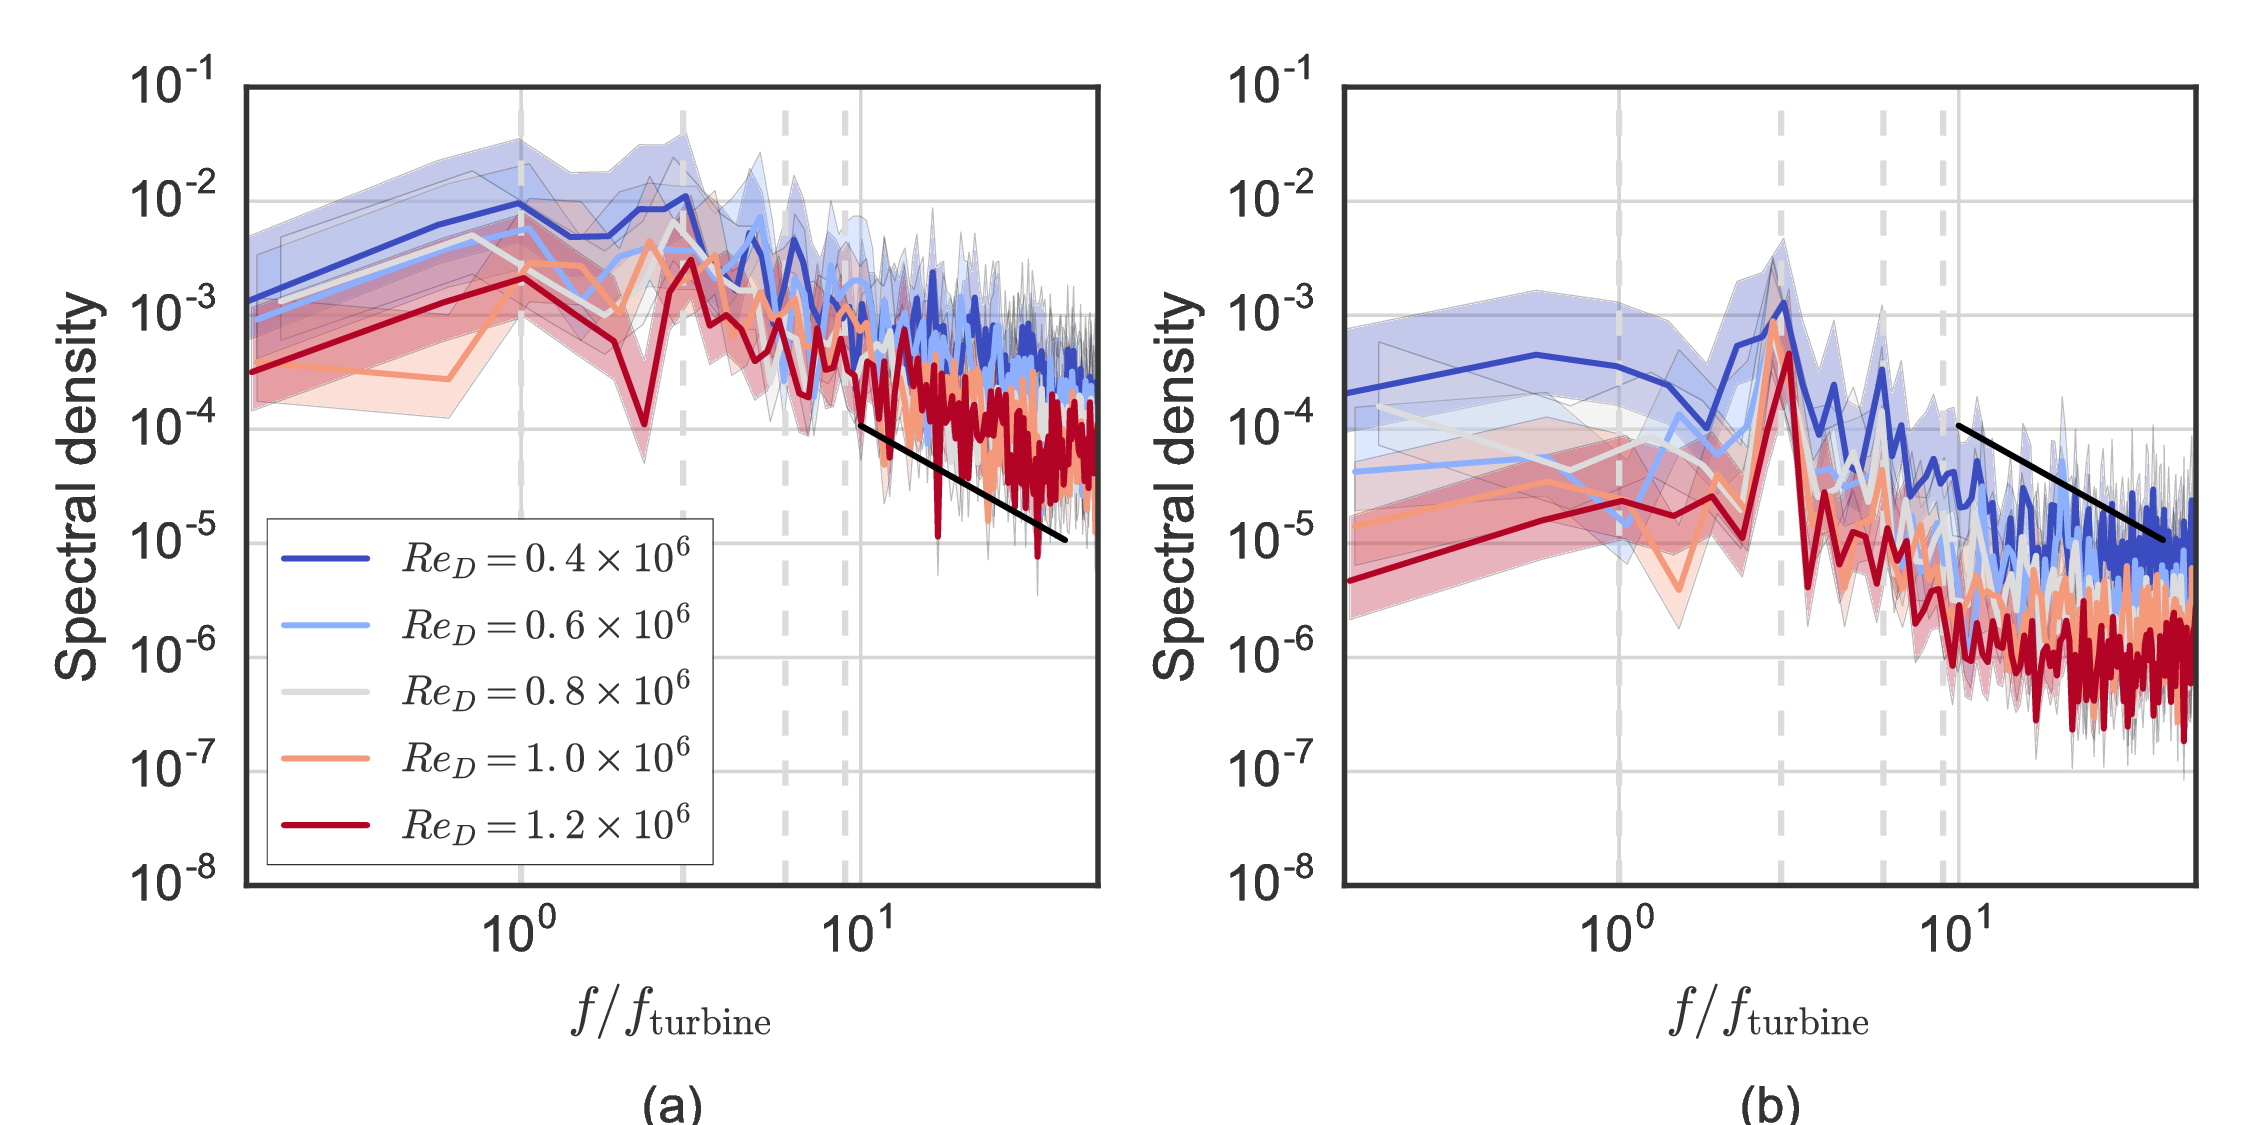
\includegraphics[width=0.85\textwidth]{RVAT-Re-dep_wake_spectra}
    
    \caption{Cross-stream velocity (normalized by $U_\infty$) spectra at
        $z/H=0.25$, $y/R=-1.0$ ($-0.5$ m in Figure~\ref{fig:wake-locations}) (a) and
        $y/R=1.5$ ($+0.75$ m in Figure~\ref{fig:wake-locations}) (b). Dashed
        vertical lines indicate $[1, 3, 6, 9]$ times the turbine rotational
        frequency. Shaded regions indicate 95\% confidence intervals assuming a
        $\chi^2$~distribution.}
    
    \label{fig:wake-spectra}
\end{figure}


\subsubsection{Transport of mean momentum and kinetic energy}

The relative importance of various physical processes on mean streamwise
momentum and kinetic energy transport/recovery in the streamwise direction were
assessed by examining the governing equations rearranged to isolate the
streamwise partial derivative ($\partial / \partial x$) for the quantities of
interest~\cite{Bachant2015-JoT}, i.e., momentum:
\begin{equation}
\begin{split}
    \frac{\p U}{\p x} = 
    \frac{1}{U} \bigg{[}
    & - V\frac{\p U}{\p y}
    - W\frac{\p U}{\p z} \\
    & -\frac{1}{\rho}\frac{\p P}{\p x} \\
    & - \frac{\p}{\p x} \overline{u'u'}
    - \frac{\p}{\p y} \overline{u'v'}
    - \frac{\p}{\p z} \overline{u'w'} \\
    & + \nu\left(\frac{\p^2 U}{\p x^2}
    + \frac{\p^2 U}{\p y^2}
    + \frac{\p^2 U}{\p z^2} \right)
    \bigg{]},
\end{split}
\label{eq:momentum}
\end{equation}
and mean kinetic energy:
\begin{equation}
\begin{split}
    \frac{\p K}{\p x}
    =
    \frac{1}{U}
    \bigg{[}
    & - \underbrace{V \frac{\p K}{\p y}}_{y\text{-adv.}}
        - \underbrace{W \frac{\p K}{\p z}}_{z\text{-adv.}}
        % Pressure work:
        - \frac{1}{\rho}\frac{\p}{\p x_j} P U_i \delta_{ij}
        % Work by viscous forces
        + \frac{\p}{\p x_j} 2 \nu U_i S_{ij} % Not sure if that's capital S...
        % Turbulent transport of K
        - \underbrace{
            \frac{1}{2}\frac{\p}{\p x_j} \overline{u_i' u_j'} U_i
        }_{\text{Turb. trans.
        }} \\
        % Production of k
        & + 
        \underbrace{
            \overline{u_i' u_j'} \frac{\p U_i}{\p x_j}
        }_{k\text{-prod.
        }}
        % Mean dissipation
        - 
        \underbrace{
            2 \nu S_{ij}S_{ij}
        }_{\text{Mean diss.
        }}
        \bigg{]},
        \label{eq:K-full}
    \end{split}
\end{equation}
where advection is abbreviated by ``adv.,'' turbulent transport by ``turb.
trans.,'' production by ``prod.,'' and dissipation by ``diss.''

Note that Equations~(\ref{eq:momentum}) and (\ref{eq:K-full}) only differ from
the typical forms of the mean momentum and mean kinetic energy equations by a
factor of $1/U$, but importantly, the other convective terms ( $\partial
U/\partial y$, $\partial U/\partial z$, and $\partial K/\partial y$, $\partial
K/\partial z$ ) are moved to the right-hand sides of the equations to illustrate
with what sign they add to the streamwise recovery of streamwise momentum or
mean kinetic energy.

Results from the terms that can be computed from the experimental data
i.e., excluding $\partial / \partial x$) from the right-hand sides of
Equations~(\ref{eq:momentum}) and (\ref{eq:K-full}) are plotted in
Figures~\ref{fig:mom-bar-graph} and \ref{fig:K-bar-graph}, respectively.
Derivatives were computed using a second order finite difference scheme, with
central differencing for interior points and inward facing schemes for the
boundaries. A weighted average for each term was then calculated based on the
grid spacing. We note that similar to \cite{Bachant2015-JoT}, the vertical
advection at this point in the wake is the dominant contributor to positive wake
recovery, caused by the unique vortex pattern created by the blade tips and
blade wakes.

\begin{figure}
    \centering
    
    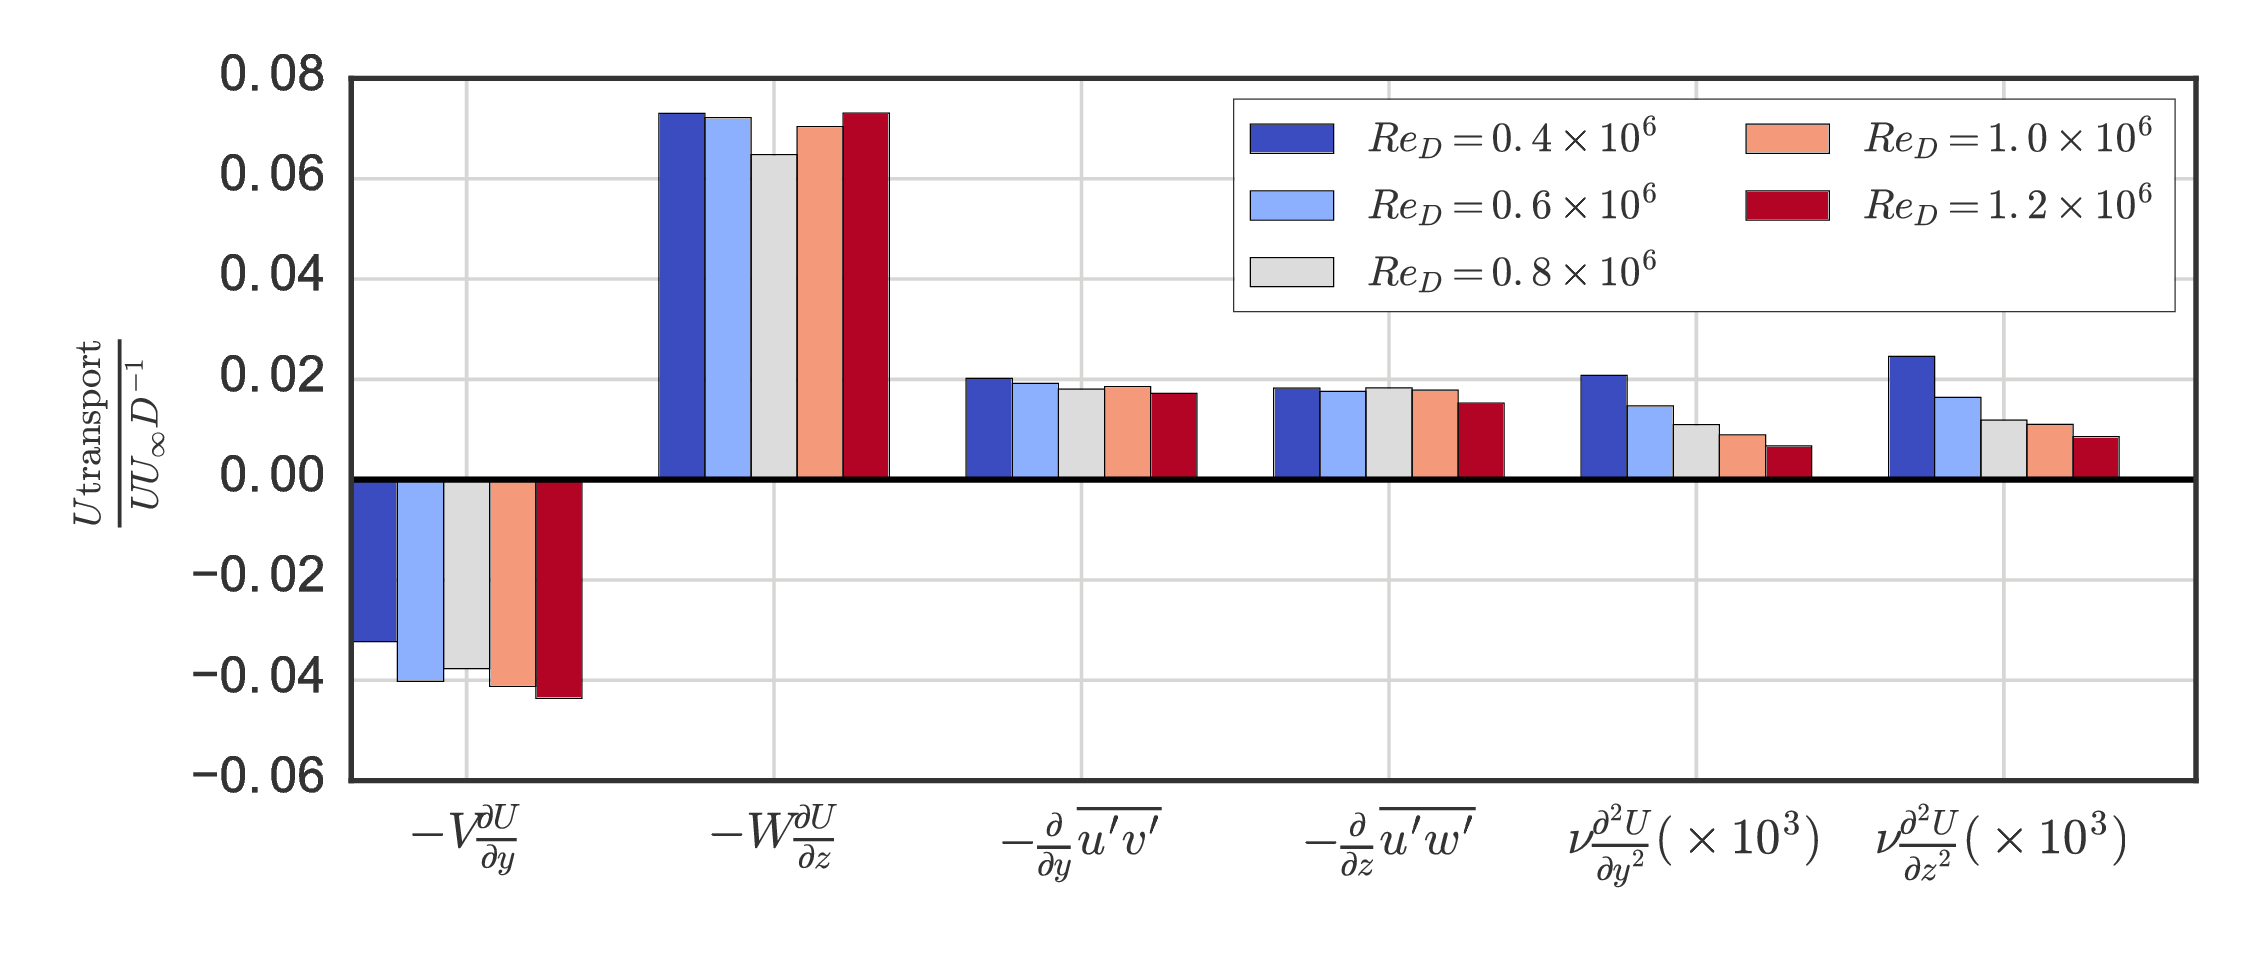
\includegraphics[width=0.9\textwidth]{RVAT-Re-dep_mom_bar_graph}
    
    \caption{Normalized streamwise momentum transport quantities computed as
        weighted averages from Equation~\ref{eq:momentum}.}
    
    \label{fig:mom-bar-graph}
\end{figure}

\begin{figure}
    \centering
    
    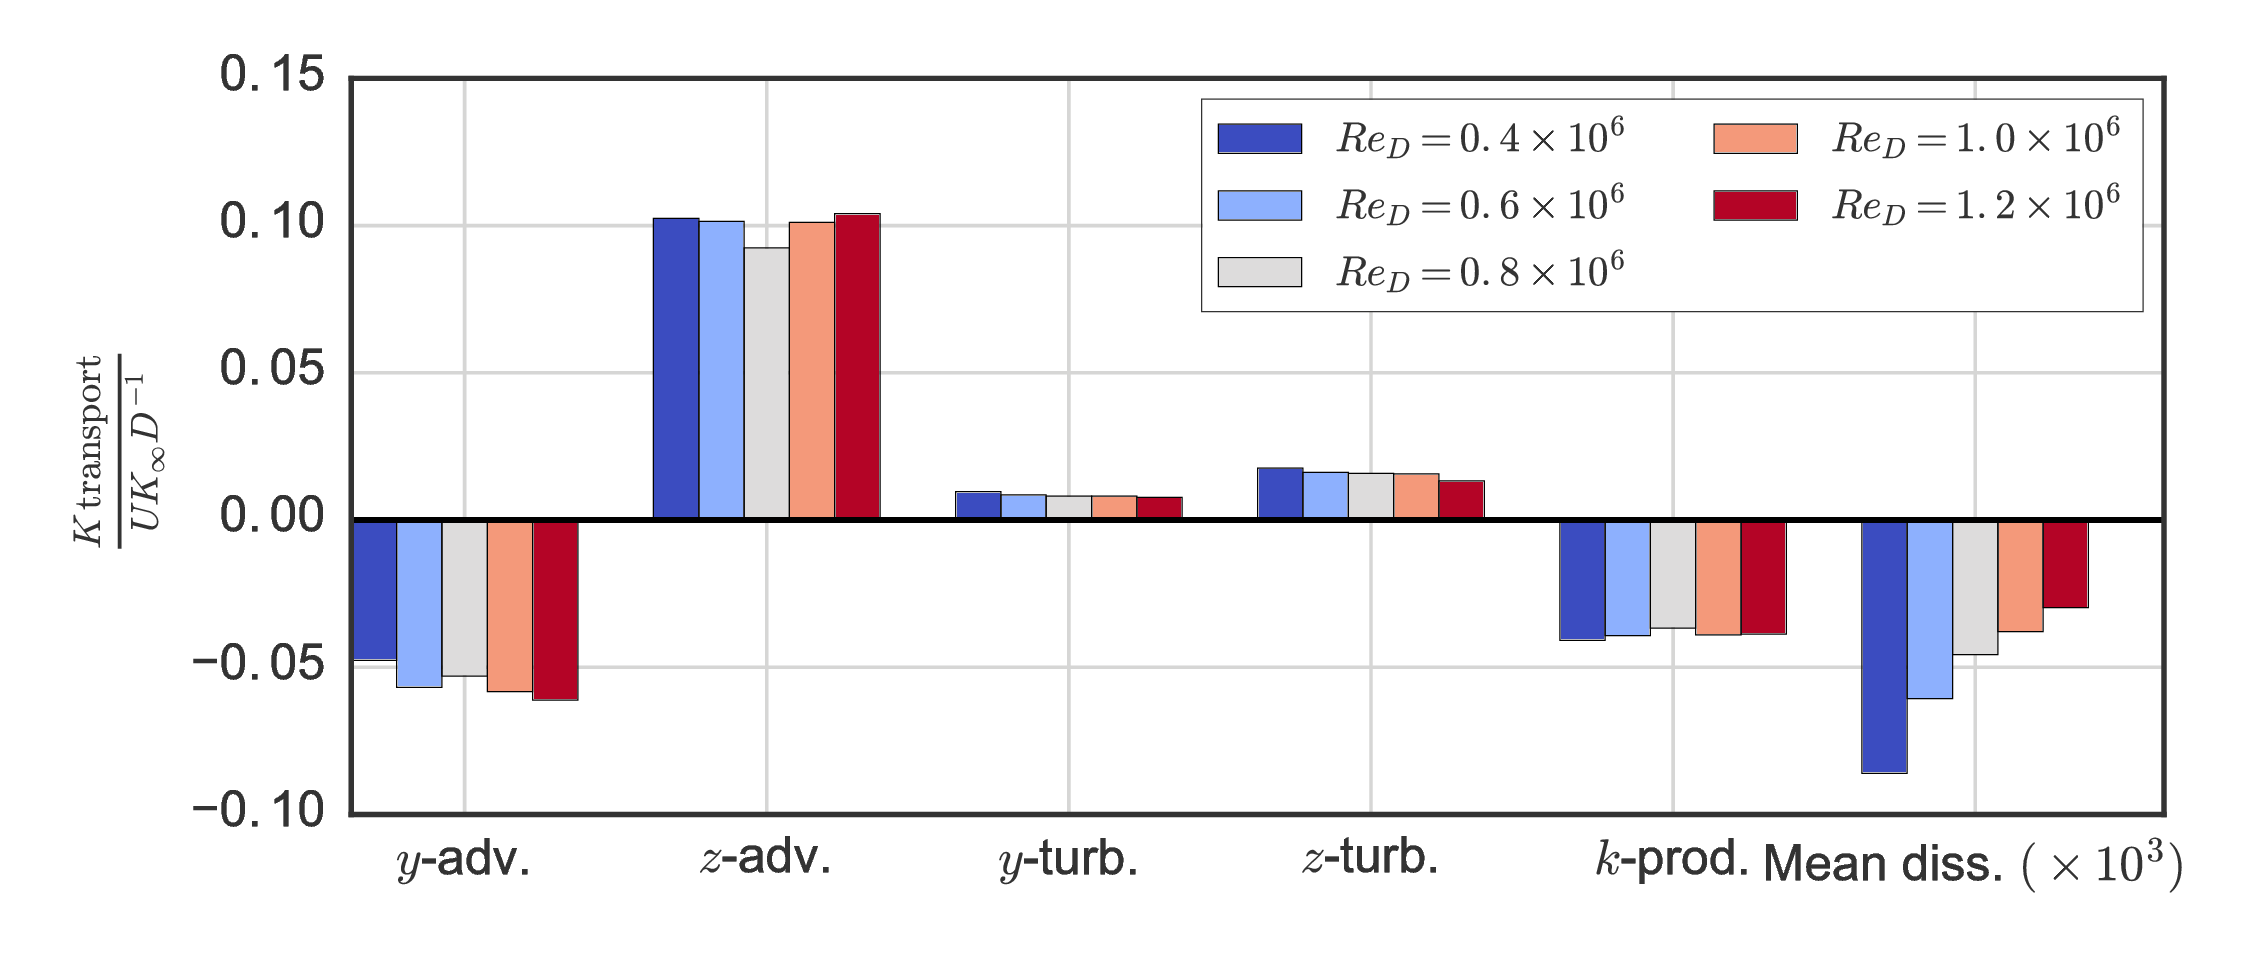
\includegraphics[width=0.9\textwidth]{RVAT-Re-dep_K_trans_bar_graph}
    
    \caption{Normalized mean kinetic energy transport quantities computed as
        weighted averages based on Equation~(\ref{eq:K-full}), omitting the
        non-measured streamwise derivatives. Note that directions of the turbulent
        transport terms refer to the directions of their partial derivatives.}
    
    \label{fig:K-bar-graph}
\end{figure}

We see that in general, levels of turbulent transport are slightly lower at
larger Reynolds numbers. The viscous diffusion and dissipation, though still
three orders of magnitude smaller than the other terms, do increase at low
Reynolds numbers, which is consistent with the physical meaning of the Reynolds
number itself. From these results, one might expect that the viscous effects
will become significant to the wake dynamics as the Reynolds number is decreased
below $Re_D \sim 10^4$.

Transport due to cross-stream advection appears to become more negative at
higher $Re$. This~could be a consequence of increasing free surface deformation
(higher $Fr$), which then decreases the effective flow cross-sectional area
downstream of the turbine, forcing more flow to accelerate around the sides of
the turbine. Note that we also observe slightly higher drag coefficients at
higher $Re$ (potentially for the same reason), which also helps explain larger
negative values of cross-stream advection.

The totals for all of the wake transport terms calculated in
Figures~\ref{fig:mom-bar-graph} and \ref{fig:K-bar-graph} are plotted in
Figure~\ref{fig:wake-trans-totals}. We see that in general, the wake transport
of both mean streamwise momentum and kinetic energy is enhanced at lower
Reynolds numbers and levels off consistent with the behavior of the turbine
power coefficient. This is an important consideration if studying sub-scale
models of turbine arrays, where increased levels of wake recovery could motivate
different ideal array configurations when compared to full-scale turbines if the
scale model Reynolds number is too low.

\begin{figure}
    \centering
    
    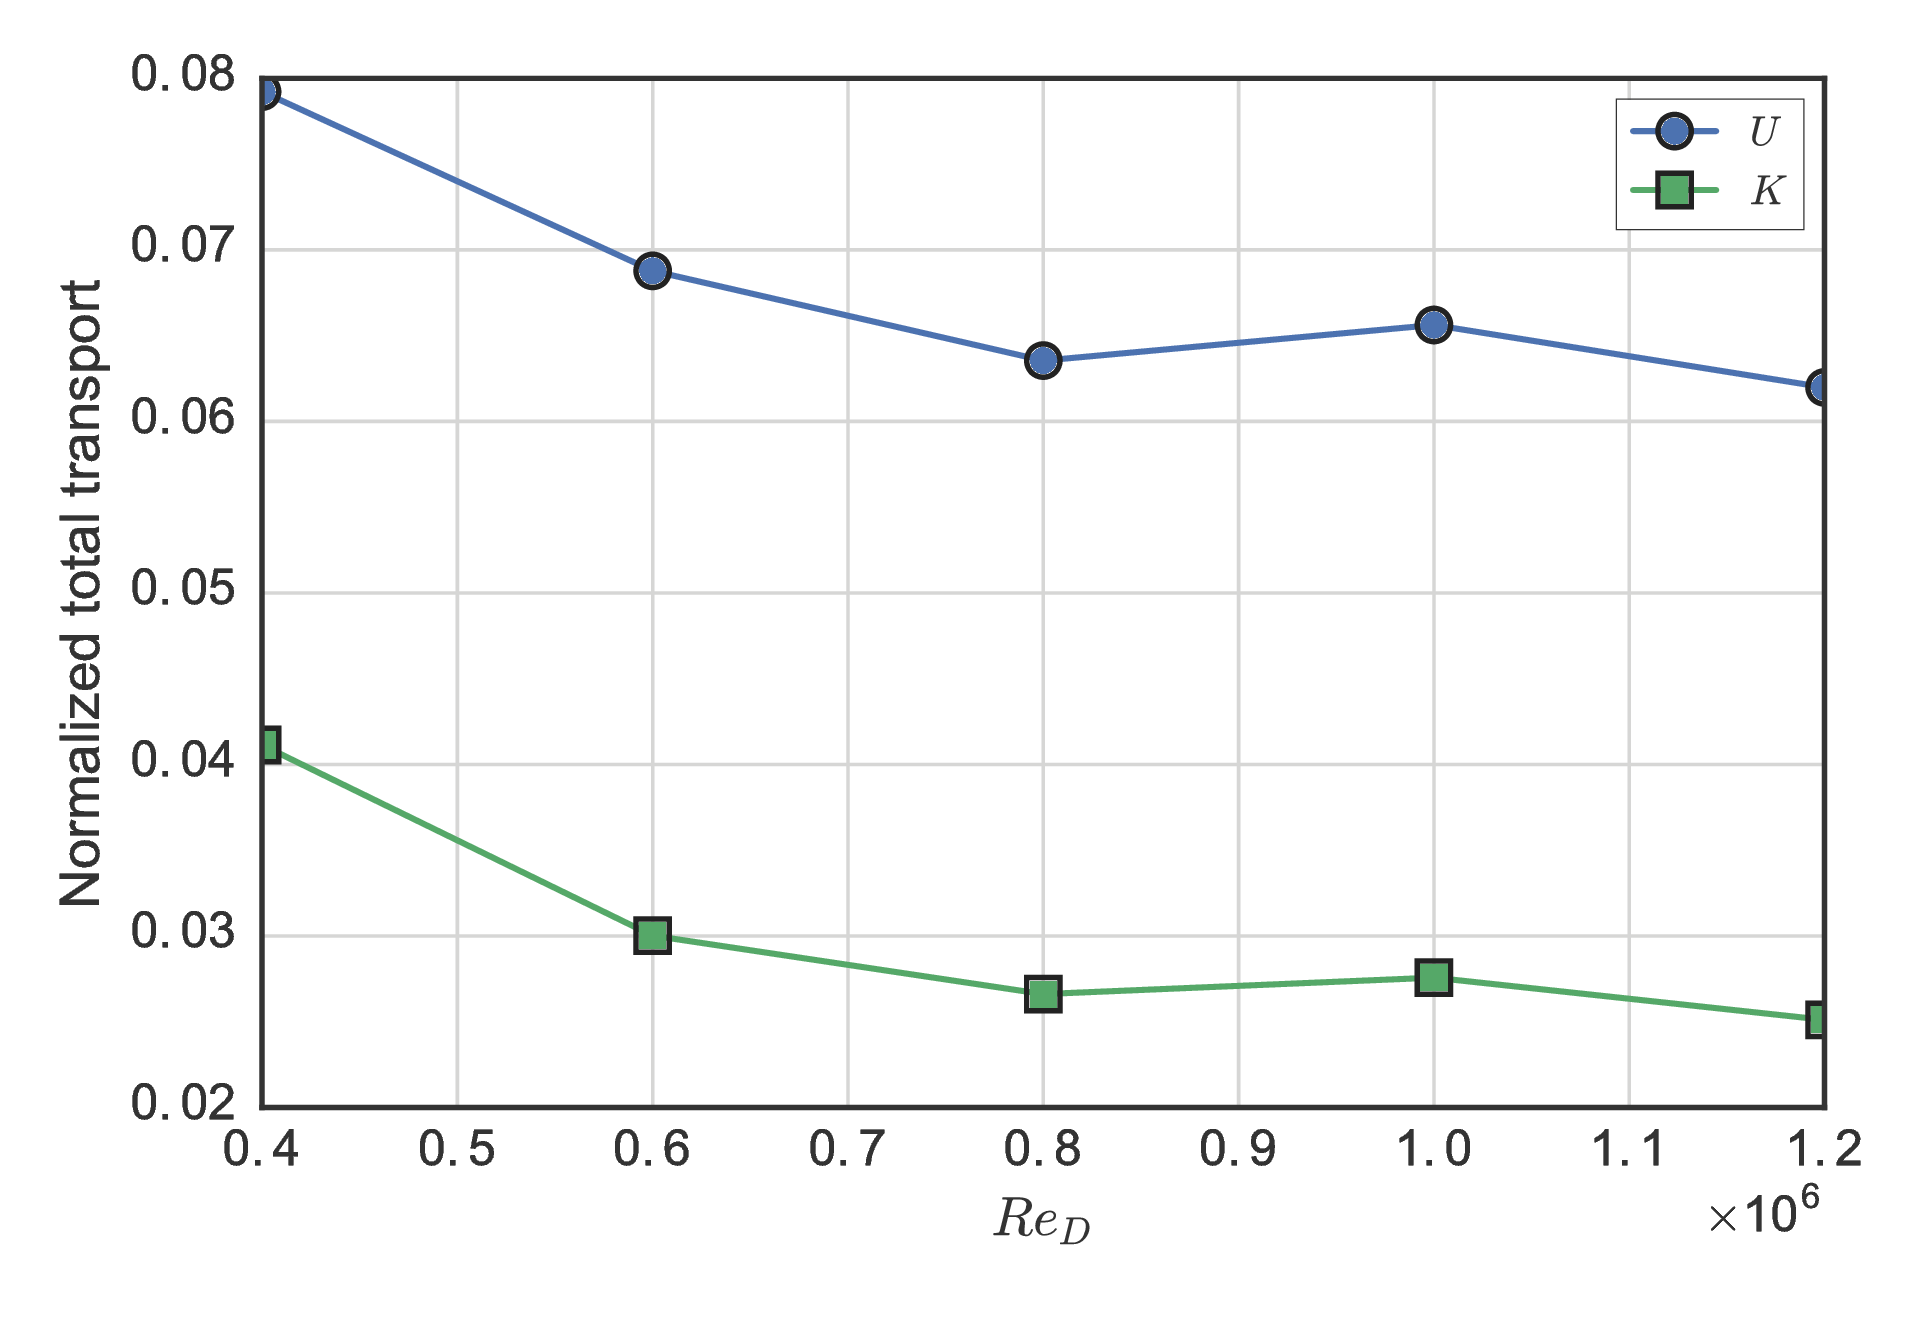
\includegraphics[width=0.75\textwidth]{RVAT-Re-dep_wake_trans_totals}
    
    \caption{Normalized transport totals from Figures~\ref{fig:mom-bar-graph}
        (streamwise momentum, $U$) and \ref{fig:K-bar-graph} (mean kinetic energy,
        $K$) plotted versus the Reynolds number.}
    
    \label{fig:wake-trans-totals}
\end{figure}

\todo[inline]{Make labels more specific.}


\section{Conclusions}

In this study, it was demonstrated that the performance of a high solidity
($c/R=0.28$) cross-flow turbine becomes essentially $Re$-independent at a
Reynolds number based on the turbine diameter $Re_D \approx 10^6$ or an
approximate Reynolds number based on the blade chord $Re_c \approx 2 \times
10^5$. The power coefficient values on the left-hand side of the $C_P$-$\lambda$
curve are reduced more than those on the right-hand side at low $Re$ due to
deeper stalling. The $Re$-independent threshold corresponds to that at which the
foil suction surface boundary layer becomes turbulent before having to recover
static pressure against the adverse pressure gradient, highlighted in
\cite{Lissaman1983, McMasters1980, Carmichael1981}.

We propose a method for predicting the Reynolds number dependence of a cross-flow
turbine using static airfoil characteristics and turbine blade kinematics:
\begin{enumerate}
    \item Acquire static lift and drag coefficient data for the desired blade
    profile.
    
    \item For azimuthal angles of 0 to 180 degrees and a given tip speed ratio,
    calculate the geometric angle of attack and relative velocity magnitude from
    the blade and undisturbed free stream velocity (taken as unity) vectors.
    
    \item With arrays of geometric angle of attack and relative velocity
    magnitude, calculate the blade chordwise force and then the rotor torque
    coefficient from Equations~(\ref{eq:ct}) and (\ref{eq:cc}), respectively.
    
    \item Extract the maximum value of $C_T$, and repeat this process for static
    foil data at multiple $Re$.
\end{enumerate}

It was shown that the peak torque coefficient computed this way shows similar
Reynolds number sensitivity as the experimental results for an actual turbine,
making it a better predictor than conventional quantifications of airfoil
performance, e.g., the lift-to-drag ratio. Note that this method is not
restricted to standard symmetrical NACA foils, though those evaluated here with
higher camber were more sensitive at lower $Re$, but had smaller slopes in the
linear~regime.

In the near-wake of the turbine, we observed lower levels of turbulence with
increasing Reynolds number, along with lower levels of turbulent transport with
respect to mean streamwise momentum and mean kinetic energy recovery in the
streamwise direction. Vertical advection, the largest transport mechanism
measured, showed little $Re$-dependence, whereas the negative effects of
cross-stream advection were enhanced at high $Re$, which may be due to larger
free surface deformation effectively reducing the near-wake's cross-sectional
area. Despite being orders of magnitude smaller than other transport processes,
viscous diffusion increased rapidly with decreasing $Re$ and is expected to
become significant to the wake dynamics around $Re_D \sim 10^4$. Overall, the
total wake transport measured leveled off at essentially the same Reynolds
number that the performance did: $Re_D \approx 0.8 \times 10^6$.

From these results, we recommend that physical model tests of cross-flow
turbines be performed at $Re_D \sim 10^6$ or greater to provide reasonable
predictions of full-scale performance. This threshold also applies to the
validation of predictive engineering models, especially for high-fidelity CFD
models where the boundary layer is to be resolved, since transition to
turbulence plays an important role in overall blade loading. Note that in our
case, blockage, though reasonably low, may be increasing flow through the
turbine compared to a free case, which could mean $Re$ thresholds for free flows
could be slightly higher, though a reliable blockage correction algorithm has
not yet been agreed upon for CFTs~\cite{Cavagnaro2014}.

If using scaled physical models to predict array performance, where turbine
power output is measured, it may also be important to keep all turbines in the
regime where the power coefficient varies linearly to avoid exaggerated power
deficiencies for downstream turbines, despite similarities in wake
characteristics. Results here also suggest that low Reynolds number physical
model studies of turbine arrays may see exaggerated levels of wake recovery,
leading to inadequate or inappropriate spacing or layouts.